\documentclass[UTF8,a4paper,11pt,fontset=fandol]{ctexart}
\newcommand{\DocTitle}{实验01\_实验讲义}
\newcommand{\DocSubject}{2026年秋季课程B：第一次实验，Python环境与基础入门}
\newcommand{\DocShortTitle}{实验一：环境与基础入门}
\newcommand{\DocType}{学生实验讲义}
% Shared style for integrated experiment handouts.
\usepackage[left=2.15cm,right=2.15cm,top=2.25cm,bottom=2.15cm,headsep=0.7cm]{geometry}
\usepackage{amsmath,amssymb}
\usepackage{booktabs,array,tabularx,longtable,multirow}
\usepackage{enumitem}
\usepackage{xcolor}
\usepackage{graphicx}
\usepackage{tikz}
\usetikzlibrary{arrows.meta,positioning,calc,shapes.geometric}
\usepackage{tcolorbox}
\usepackage{listings}
\usepackage{hyperref}
\usepackage{fancyhdr}
\usepackage{chngcntr}

\definecolor{Ink}{HTML}{17233C}
\definecolor{Navy}{HTML}{173B68}
\definecolor{Blue}{HTML}{2878B5}
\definecolor{Cyan}{HTML}{2A9D8F}
\definecolor{Amber}{HTML}{E9A23B}
\definecolor{Red}{HTML}{C84B4B}
\definecolor{Paper}{HTML}{F6F8FB}
\definecolor{PaleBlue}{HTML}{EAF2FA}
\definecolor{PaleCyan}{HTML}{EAF7F4}
\definecolor{PaleAmber}{HTML}{FFF5E4}
\definecolor{Rule}{HTML}{D6DEE8}
\definecolor{Muted}{HTML}{5B677A}

\hypersetup{
  colorlinks=true,
  linkcolor=Navy,
  urlcolor=Blue,
  citecolor=Cyan,
  pdfauthor={《人工智能数学原理与算法》课程组},
  pdftitle={\DocTitle},
  pdfsubject={\DocSubject}
}

\ctexset{
  section={format=\Large\bfseries\color{Navy},beforeskip=1.4ex plus .2ex,afterskip=.8ex},
  subsection={format=\large\bfseries\color{Ink},beforeskip=1.2ex plus .2ex,afterskip=.55ex},
  subsubsection={format=\normalsize\bfseries\color{Blue},beforeskip=1ex,afterskip=.35ex}
}

\setlength{\parindent}{2em}
\setlength{\parskip}{0.22em}
\setlength{\emergencystretch}{2em}
\linespread{1.14}
\setlist[itemize]{leftmargin=2em,itemsep=.25em,topsep=.35em}
\setlist[enumerate]{leftmargin=2.2em,itemsep=.28em,topsep=.35em}
\renewcommand{\arraystretch}{1.30}
\newcolumntype{Y}{>{\raggedright\arraybackslash}X}
\newcolumntype{C}[1]{>{\centering\arraybackslash}p{#1}}
\newcolumntype{L}[1]{>{\raggedright\arraybackslash}p{#1}}

\newcommand{\R}{\mathbb{R}}
\newcommand{\E}{\mathbb{E}}
\newcommand{\MSE}{\operatorname{MSE}}
\newcommand{\RMSE}{\operatorname{RMSE}}
\newcommand{\argmin}{\operatorname*{arg\,min}}
\newcommand{\vect}[1]{\boldsymbol{#1}}
\newcommand{\mat}[1]{\mathbf{#1}}
\newcommand{\term}[1]{\textcolor{Blue}{\textbf{#1}}}
\newcommand{\code}[1]{\texttt{#1}}
\numberwithin{equation}{subsection}

\tcbset{boxrule=.7pt,arc=1.6mm,left=2.5mm,right=2.5mm,top=1.8mm,bottom=1.8mm,before skip=7pt,after skip=7pt}
\newtcolorbox{keybox}[1][核心结论]{colback=PaleBlue,colframe=Blue,title={#1},fonttitle=\bfseries,coltitle=Ink}
\newtcolorbox{examplebox}[1][贯穿例题]{colback=PaleCyan,colframe=Cyan,title={#1},fonttitle=\bfseries,coltitle=Ink}
\newtcolorbox{questionbox}[1][检查点]{colback=PaleAmber,colframe=Amber,title={#1},fonttitle=\bfseries,coltitle=Ink}
\newtcolorbox{pitfallbox}[1][易错提醒]{colback=red!3,colframe=Red,title={#1},fonttitle=\bfseries,coltitle=Ink}
\newtcolorbox{teacherbox}[1][教师提示]{colback=Paper,colframe=Rule,title={#1},fonttitle=\bfseries,coltitle=Muted}
\newtcolorbox{proofbox}[1][推导与证明]{colback=Blue!3,colframe=Navy,title={#1},fonttitle=\bfseries,coltitle=Ink}

\lstdefinestyle{python}{
  language=Python,
  basicstyle=\ttfamily\small,
  keywordstyle=\color{Blue}\bfseries,
  commentstyle=\color{Cyan!70!black},
  stringstyle=\color{Red!80!black},
  showstringspaces=false,
  columns=fullflexible,
  keepspaces=true,
  frame=single,
  rulecolor=\color{Rule},
  backgroundcolor=\color{Paper},
  breaklines=true,
  numbers=left,
  numberstyle=\tiny\color{Muted},
  xleftmargin=1.5em,
  framexleftmargin=1.2em,
  aboveskip=.7em,
  belowskip=.7em
}
\lstset{style=python}

\pagestyle{fancy}
\fancyhf{}
\fancyhead[L]{\small\color{Muted}人工智能数学原理与算法}
\fancyhead[R]{\small\color{Muted}\DocShortTitle}
\fancyfoot[L]{\small\color{Muted}\DocType}
\fancyfoot[R]{\small\color{Muted}\thepage}
\renewcommand{\headrulewidth}{0pt}
\renewcommand{\footrulewidth}{0pt}

\newcommand{\makeexperimenttitle}[4]{
  \hypersetup{pageanchor=false}
  \begin{titlepage}\thispagestyle{empty}
  \begin{tikzpicture}[remember picture,overlay]
    \fill[Ink] (current page.north west) rectangle ([yshift=-9.4cm]current page.north east);
    \fill[Blue] ([yshift=-9.4cm]current page.north west) rectangle ([yshift=-9.68cm]current page.north east);
    \fill[Cyan] ([xshift=2.15cm,yshift=-1.55cm]current page.north west) rectangle ([xshift=2.27cm,yshift=-8.55cm]current page.north west);
    \fill[Paper] ([xshift=2.15cm,yshift=2.0cm]current page.south west) rectangle ([xshift=-2.15cm,yshift=6.15cm]current page.south east);
  \end{tikzpicture}
  \vspace*{1.45cm}
  {\color{white}\Large 人工智能数学原理与算法\par}\vspace{.55cm}
  {\color{white}\fontsize{31}{39}\selectfont\bfseries #1\par}\vspace{.35cm}
  {\color{white}\fontsize{21}{28}\selectfont #2\par}
  \vfill
  \begin{tcolorbox}[colback=white,colframe=white,boxrule=0pt,arc=0mm,left=7mm,right=7mm,top=6mm,bottom=6mm,width=\textwidth]
    \begin{tabularx}{\linewidth}{L{2.6cm}Y}
      \textcolor{Muted}{材料类型} & \DocType\\
      \textcolor{Muted}{实验安排} & #3\\
      \textcolor{Muted}{贯穿案例} & #4\\
      \textcolor{Muted}{适用对象} & 已完成机器学习导论、具备高中数学与基础计算机操作能力的本科生\\
    \end{tabularx}
  \end{tcolorbox}
  \vspace{.7cm}{\color{Muted}\small 版本：2026年秋季学期整合稿\hfill 源文件与 PDF 同目录交付\par}
  \end{titlepage}
  \hypersetup{pageanchor=true}
  \pagenumbering{roman}\tableofcontents\clearpage\pagenumbering{arabic}
}

\usepackage{calc}
\usepackage{etoolbox}
\usepackage{xurl}
\usepackage{bookmark}
\setmonofont[BoldFont=DejaVuSansMono-Bold.ttf,ItalicFont=DejaVuSansMono-Oblique.ttf,BoldItalicFont=DejaVuSansMono-BoldOblique.ttf]{DejaVuSansMono.ttf}
\setCJKmonofont[AutoFakeBold=2]{FandolFang-Regular.otf}
% Pandoc's captionless longtables use this counter with TeX Live 2024.
\newcounter{none}
\providecommand{\tightlist}{\setlength{\itemsep}{0pt}\setlength{\parskip}{0pt}}
\providecommand{\passthrough}[1]{#1}
\providecommand{\pandocbounded}[1]{#1}
\setcounter{tocdepth}{1}
\setcounter{secnumdepth}{2}
\setlength{\headheight}{15pt}
\lstset{basicstyle=\ttfamily\small,numbers=none,xleftmargin=0pt,framexleftmargin=0pt,breakatwhitespace=false}
\AtBeginEnvironment{longtable}{\small\setlength{\tabcolsep}{4pt}}
\hypersetup{hypertexnames=false,pdfauthor={钟志诚（主讲）；曾有成、史睿铭、胡泷（整理）}}
\begin{document}
\raggedright
\setlength{\parindent}{2em}
\hypersetup{pageanchor=false}
\begin{titlepage}
\thispagestyle{empty}
\vspace*{1.5cm}
{\Large\color{Navy}人工智能数学原理与算法 B\par}
\vspace{1cm}
{\huge\bfseries\color{Ink}第一次实验\par}
\vspace{.45cm}
{\LARGE\bfseries\color{Ink}Python 环境与基础入门\par}
\vspace{.6cm}
{\Large 学生实验讲义\par}
\vspace{1cm}
{\large 2026 年秋季学期\par}
\vspace{.8cm}
\begin{tabular}{@{}ll}
主讲 & 钟志诚\\[.35em]
整理 & 曾有成、史睿铭、胡泷\\[.35em]
单位 & 中国科学技术大学\\
     & 人工智能与数据科学学院
\end{tabular}
\vspace{1cm}\par
建议课前完成环境安装与首次运行。\\
日期、地点与提交平台以课程通知为准。\par
\vfill
\noindent\rule{\linewidth}{.5pt}\par
微型书店：对象、继承、数据管理与销售统计。\\
鸢尾花：补全模型调用，完成训练与结果验证。\\
基础练习 Notebook 配合教学，不要求提交。\par
\end{titlepage}
\hypersetup{pageanchor=true}
\pagenumbering{roman}
\tableofcontents
\clearpage
\pagenumbering{arabic}
\section{从 C 语言到 Python}\label{ux4ece-c-ux8bedux8a00ux5230-python}

\subsection{从已有的编程经验出发}\label{ux4eceux5df2ux6709ux7684ux7f16ux7a0bux7ecfux9a8cux51faux53d1}

在 C 语言中，我们已经接触过用变量保存数据、用条件判断和循环控制程序执行，以及用函数组织可以重复使用的代码。这些基本思路在 Python 中仍然适用。学习 Python 时，可以从熟悉的程序出发，比较相同的计算过程在两种语言中如何表达。

本次实验以书店中的图书信息为例。计算购书费用，需要保存单价和数量；筛选有货的图书，需要逐条检查库存；统计库存总值，则需要重复计算并累加。我们将借助这些例子回顾已有的编程方法，熟悉 Python 的写法，并认识列表、字典等组织数据的方式。例中的书名、价格、库存与销量均为人工构造的教学数据，便于手工核对计算结果。

随后，实验将引入 NumPy 数组，处理一批数值的计算；通过类组织相关的数据和操作；最后调用 scikit-learn，完成数据准备、模型训练与预测的基本流程。分类部分先学习如何使用已有模型，算法内部的数学计算将在后续实验中展开。

环境安装与运行方法见实验手册。建议课前完成安装和首次运行。完成安装后，先运行下面的小程序，确认代码由哪个 Python 解释器执行。

\subsection{文件、解释器与运行结果}\label{ux6587ux4ef6ux89e3ux91caux5668ux4e0eux8fd0ux884cux7ed3ux679c}

此前运行 C 程序时，通常需要先将源文件编译为可执行文件。运行本课的 Python 脚本时，把保存代码的 \passthrough{\lstinline!.py!} 文件交给 Python 解释器即可。例如，将代码保存为 \passthrough{\lstinline!hello.py!} 后，在该目录的终端输入 \passthrough{\lstinline!python hello.py!}，就是让 Python 执行这个文件。编辑器用于修改文件，终端用于输入运行命令。

另一种方式是打开 \passthrough{\lstinline!.ipynb!} 格式的 Jupyter Notebook。Notebook 将说明文字、代码和输出放在一起，由内核执行代码单元。\passthrough{\lstinline!practice.ipynb!} 配合讲义练习基础操作，不要求提交。正式作业分别在 \passthrough{\lstinline!code/bookstore!} 和 \passthrough{\lstinline!code/iris!} 中完成，各目录的 README 说明补全位置与运行方法。下面的 Python 代码可以写在脚本或 Notebook 代码单元中；上面的运行命令则在终端中输入。

\begin{lstlisting}[language=Python]
import sys
print(sys.executable)
print("你好，Python！")
\end{lstlisting}

\passthrough{\lstinline!print!} 将内容显示出来，作用上可以联系 C 中的输出函数。这里先用 \passthrough{\lstinline!import sys!} 导入 Python 的标准库模块 \passthrough{\lstinline!sys!}，再读取 \passthrough{\lstinline!sys.executable!}，显示当前解释器的位置。电脑上可能有多个 Python 环境，这个路径可以帮助我们核对程序是否正在课程环境中运行。第二行输出是问候语。

\textbf{检查点 C1：} 修改问候语，保存并重新运行。你改的是文件中的哪一行？输出是否真的改变？

Notebook 的内核会保留已执行单元产生的变量和函数。修改代码后，需要重新执行相应单元，内核中的状态才会更新；例如修改函数后，要先运行函数定义单元，再运行调用它的单元。

\clearpage

\section{变量与容器：把问题写成数据}\label{ux53d8ux91cfux4e0eux5bb9ux5668ux628aux95eeux9898ux5199ux6210ux6570ux636e}

\subsection{变量、数值与字符串}\label{ux53d8ux91cfux6570ux503cux4e0eux5b57ux7b26ux4e32}

一本书单价 32 元，购买两本，总价为 64 元。在 C 语言中，可以先用 \passthrough{\lstinline!double price = 32.0;!} 和 \passthrough{\lstinline!int quantity = 2;!} 定义单价与数量，再计算它们的乘积。Python 中可以这样写：

\begin{lstlisting}[language=Python]
title = "星空旅行"
price = 32.0
quantity = 2
in_stock = True
total = price * quantity
print(title, total)
\end{lstlisting}

运行后显示 \passthrough{\lstinline!星空旅行 64.0!}。乘法与赋值的写法和 C 语言相近；这里用 \passthrough{\lstinline!print!} 显示结果，每条语句末尾不需要分号。\passthrough{\lstinline!=!} 用于赋值，\passthrough{\lstinline!==!} 用于比较是否相等，变量名仍区分大小写。

Python 的赋值语句不需要在变量名前声明类型。上例中的 \passthrough{\lstinline!32.0!} 是浮点数 \passthrough{\lstinline!float!}，\passthrough{\lstinline!2!} 是整数 \passthrough{\lstinline!int!}，带引号的 \passthrough{\lstinline!"星空旅行"!} 是字符串 \passthrough{\lstinline!str!}。\passthrough{\lstinline!in\_stock!} 保存布尔值 \passthrough{\lstinline!True!}，表示有货；表示无货时可以用 \passthrough{\lstinline!False!}。这两个布尔值的首字母均大写。

类型仍然影响运算的含义。\passthrough{\lstinline!32.0 + 32.0!} 得到数值 \passthrough{\lstinline!64.0!}，而 \passthrough{\lstinline!"32.0" + "32.0"!} 得到拼接后的字符串 \passthrough{\lstinline!"32.032.0"!}。可以用 \passthrough{\lstinline!type(price)!} 查看类型，用 \passthrough{\lstinline!float("32.0")!} 将表示数值的文本转换为浮点数。后面从文件读取价格时，还会用到这种转换。

数值的加、减、乘分别使用 \passthrough{\lstinline!+!}、\passthrough{\lstinline!-!}、\passthrough{\lstinline!*!}。除法需要留意与 C 整数运算的区别：Python 中 \passthrough{\lstinline!5 / 2!} 得到 \passthrough{\lstinline!2.5!}，\passthrough{\lstinline!5 // 2!} 得到 \passthrough{\lstinline!2!}，其中 \passthrough{\lstinline!//!} 表示向下取整的除法。余数使用 \passthrough{\lstinline!\%!}，乘方使用 \passthrough{\lstinline!**!}，例如 \passthrough{\lstinline!2 ** 3!} 得到 \passthrough{\lstinline!8!}。

\textbf{检查点 C2：} 不运行先预测 \passthrough{\lstinline!"3" + "2"!}、\passthrough{\lstinline!3 + 2!}、\passthrough{\lstinline!3 * 2!} 的结果，再运行核对。把购买册数改成 3，预期总价是多少？

\clearpage

\subsection{列表按位置找，字典按名字找}\label{ux5217ux8868ux6309ux4f4dux7f6eux627eux5b57ux5178ux6309ux540dux5b57ux627e}

只有一本书时，几个变量就能保存所需信息。书目增加后，我们需要把相关的数据组织起来。

先考虑几本书的书名。在 C 语言中，我们接触过用数组按位置访问多个元素。Python 的列表也支持按位置取值，下标同样从 0 开始：

\begin{lstlisting}[language=Python]
titles = ["星空旅行", "山间日记", "海边故事"]
print(titles[0])
print(titles[0:2])
print(len(titles))
\end{lstlisting}

三行输出依次为第一本书的书名、前两本书组成的列表，以及元素个数 \passthrough{\lstinline!3!}。切片 \passthrough{\lstinline!titles[0:2]!} 取出下标从 0 开始、到 2 之前的元素，包含下标 0 和 1。这个列表的有效非负下标是 0、1、2，访问 \passthrough{\lstinline!titles[3]!} 会越界。

这里可以借助数组理解按下标访问的方式；Python 列表的长度可以改变，也可以保存不同类型的元素，与 C 数组的类型和存储规则有所不同。

一本书还包含价格和库存。我们可以用字典把这些信息放在一起，用键说明每个值的含义：

\begin{lstlisting}[language=Python]
book = {"title": "星空旅行", "price": 32.0, "stock": 5}
print(book["price"])
\end{lstlisting}

\passthrough{\lstinline!book["price"]!} 得到 \passthrough{\lstinline!32.0!}。列表通过下标访问元素，字典通过键查找对应的值；本例使用 \passthrough{\lstinline!"title"!}、\passthrough{\lstinline!"price"!} 和 \passthrough{\lstinline!"stock"!} 三个字符串作为键。

把每本书写成一条字典记录，再将这些记录放进列表，就得到了后续程序使用的书目：

\begin{lstlisting}[language=Python]
books = [
    {"title": "星空旅行", "price": 32.0, "stock": 5},
    {"title": "山间日记", "price": 25.0, "stock": 0},
    {"title": "海边故事", "price": 18.0, "stock": 3},
]
\end{lstlisting}

这份书目对应以下数据：

\begin{longtable}[]{@{}lrr@{}}
\toprule\noalign{}
书名 & 单价（元） & 库存（册） \\
\midrule\noalign{}
\endhead
\bottomrule\noalign{}
\endlastfoot
星空旅行 & 32.0 & 5 \\
山间日记 & 25.0 & 0 \\
海边故事 & 18.0 & 3 \\
\end{longtable}

读取第一本书的库存可以写成 \passthrough{\lstinline!books[0]["stock"]!}。其中，\passthrough{\lstinline!books[0]!} 先取出第一条记录，后面的 \passthrough{\lstinline!["stock"]!} 再从这条记录中取出库存，结果为 \passthrough{\lstinline!5!}。

\textbf{检查点 C3：} 第一条记录的库存怎样取出？把第二条记录的库存改为 2，后面的有货判断会怎样变化？完成修改实验后恢复原始数据，以便与给定预期结果比较。

\clearpage

\subsection{从记录到多维数据 *}\label{ux4eceux8bb0ux5f55ux5230ux591aux7ef4ux6570ux636e}

* 表示选读内容。

前面用字典保存一本书的信息，用列表组织多本书的记录。进行数值计算时，我们还可以从记录中取出所需的数值，按明确的顺序排列。例如，三本书的价格可以排成一列，三天的销量可以排成一张表。随着数据增加，程序需要知道每个位置对应哪本书、哪一天，以及哪家书店。

本节先认识这些数据的组织方式。代码使用第 6 章将介绍的 NumPy，可以先阅读例子，在完成 NumPy 安装与导入后再运行。

\subsubsection{形状记录了什么}\label{ux5f62ux72b6ux8bb0ux5f55ux4e86ux4ec0ux4e48}

教材附录 A 用向量表示一组有序的数，用矩阵表示按行、列组织的数。在机器学习编程中，标量、向量和矩阵的数值表示还可以推广到具有更多轴的数组，统称为张量数据。定位其中一个元素时，需要沿每个轴指定位置；形状则记录各轴的长度。本节用 NumPy 数组演示这种表示方式，后续使用 PyTorch 时会接触它的 \passthrough{\lstinline!Tensor!} 类型。

\begin{longtable}[]{@{}lll@{}}
\toprule\noalign{}
数据 & 各轴的含义 & 形状示例 \\
\midrule\noalign{}
\endhead
\bottomrule\noalign{}
\endlastfoot
一本书的价格 & 无轴，单个数值 & \passthrough{\lstinline!()!} \\
三本书的价格 & 图书 & \passthrough{\lstinline!(3,)!} \\
三天中三本书的销量 & 日期、图书 & \passthrough{\lstinline!(3, 3)!} \\
两家书店的上述销量 & 书店、日期、图书 & \passthrough{\lstinline!(2, 3, 3)!} \\
\end{longtable}

这里 \passthrough{\lstinline!(3,)!} 表示一个轴、长度为 3。数学上含三个分量的向量可以称为三维向量；在数组表示中，它可以是只有一个轴的一维数组。``向量有几个分量''和``数组有几个轴''说的是不同的事情。

\begin{lstlisting}[language=Python]
import numpy as np

prices = np.array([32.0, 25.0, 18.0])
print(prices.shape)  # (3,)
print(prices.ndim)   # 1
\end{lstlisting}

\passthrough{\lstinline!shape!} 给出形状，\passthrough{\lstinline!ndim!} 给出轴的数量。它们描述结构；每个轴代表什么，还需要结合数据来源说明。列表和字典中混合的书名、价格与库存，也不能仅通过换一个类型名就获得适合模型计算的数值表示。

\clearpage

\subsubsection{图像为什么有通道轴}\label{ux56feux50cfux4e3aux4ec0ux4e48ux6709ux901aux9053ux8f74}

在前馈神经网络章节，我们讨论过如何使用卷积处理图像的局部区域。在后续的可选实验``基于 CNN 的图像分类''中，也会涉及图像、NumPy 数组与张量之间的具体转换。我们将在这个具体的主题下，介绍张量的主要操作。

先从常规的 RGB 三通道图像开始，并仅考虑 2×2 的分辨率。每个像素由红、绿、蓝三个分量组成，下面依次放置红色、绿色、蓝色和白色四个像素：

\begin{lstlisting}[language=Python]
image_hwc = np.array([
    [[255, 0, 0], [0, 255, 0]],
    [[0, 0, 255], [255, 255, 255]],
], dtype=np.uint8)

print(image_hwc.shape)    # (2, 2, 3)
print(image_hwc[0, 1])    # [  0 255   0]
\end{lstlisting}

三个轴依次是高度 \passthrough{\lstinline!H!}、宽度 \passthrough{\lstinline!W!} 和颜色通道 \passthrough{\lstinline!C!}。\passthrough{\lstinline!image\_hwc[0, 1]!} 取出第一行第二列像素的三个颜色分量。\passthrough{\lstinline!uint8!} 表示无符号 8 位整数，适合保存本例中 0 到 255 的分量值。

图像模型还可能要求通道在前，用 \passthrough{\lstinline!C、H、W!} 的顺序接收一张图像。调整轴顺序时，应同时保持各个数值对应的像素与通道不变：

\begin{lstlisting}[language=Python]
image_chw = image_hwc.transpose(2, 0, 1)
print(image_chw.shape)    # (3, 2, 2)
print(image_chw[:, 0, 1]) # [  0 255   0]

image_float = image_chw.astype(np.float32) / 255.0
print(image_float[:, 0, 1])  # [0. 1. 0.]
\end{lstlisting}

\passthrough{\lstinline!transpose(2, 0, 1)!} 将原来的第 2 个轴放到最前，原来的第 0、1 个轴随后排列。像素的含义保持不变。其中，\passthrough{\lstinline!astype(np.float32)!} 转换数值类型，除以 \passthrough{\lstinline!255.0!} 将取值范围缩放到 0 到 1。换轴、类型转换和数值缩放分别完成不同的工作。

多张相同形状的图像可以沿一个新的轴组合成批次。下面为了观察形状，将同一张小图重复放置两次：

\begin{lstlisting}[language=Python]
batch = np.stack([image_float, image_float], axis=0)
print(batch.shape)  # (2, 3, 2, 2)
\end{lstlisting}

四个轴依次对应图像数量、通道、高度和宽度，常记为 \passthrough{\lstinline!N、C、H、W!}。这里的 \passthrough{\lstinline!N=2!} 表示批次中有两张图。实验指导书中的 MNIST 和 CIFAR-10 任务也需要检查批次与通道，但实际采用的轴顺序应以模型接口为准。

\clearpage

\subsubsection{改变形状与交换轴}\label{ux6539ux53d8ux5f62ux72b6ux4e0eux4ea4ux6362ux8f74}

在连接模型的不同部分时，有时需要将一组数重新分组，有时需要改变各轴的位置。仅检查输出形状，可能无法发现这两种操作的区别：

\begin{lstlisting}[language=Python]
a = np.array([[1, 2, 3],
              [4, 5, 6]])

print(a.reshape(3, 2))
# [[1 2]
#  [3 4]
#  [5 6]]

print(a.transpose(1, 0))
# [[1 4]
#  [2 5]
#  [3 6]]
\end{lstlisting}

两个结果都是三行两列。这里 \passthrough{\lstinline!reshape!} 按默认的元素遍历顺序重新分组，转置则交换行与列的角色。因而，将图像从 \passthrough{\lstinline!H、W、C!} 排列改为 \passthrough{\lstinline!C、H、W!} 时，不能用 \passthrough{\lstinline!reshape(C, H, W)!} 代替换轴。

\textbf{想一想：} 上例中，原数组第一行第二列的数值 \passthrough{\lstinline!2!}，经过两种操作后分别位于哪里？如果把图像的通道与空间位置弄混，形状正确是否就足以说明输入正确？

\subsubsection{在后续专题中继续使用}\label{ux5728ux540eux7eedux4e13ux9898ux4e2dux7ee7ux7eedux4f7fux7528}

图像之外，表格、文本和语音也需要先明确数据各轴的含义，再决定转换方式。以下是实验指导书中可以继续观察的例子：

\begin{longtable}[]{@{}
  >{\raggedright\arraybackslash}p{(\linewidth - 4\tabcolsep) * \real{0.3333}}
  >{\raggedright\arraybackslash}p{(\linewidth - 4\tabcolsep) * \real{0.3333}}
  >{\raggedright\arraybackslash}p{(\linewidth - 4\tabcolsep) * \real{0.3333}}@{}}
\toprule\noalign{}
\begin{minipage}[b]{\linewidth}\raggedright
专题
\end{minipage} & \begin{minipage}[b]{\linewidth}\raggedright
数据组织与转换
\end{minipage} & \begin{minipage}[b]{\linewidth}\raggedright
可以先关注的问题
\end{minipage} \\
\midrule\noalign{}
\endhead
\bottomrule\noalign{}
\endlastfoot
第 1 章逻辑回归 & 将表格中的输入特征与标签分开，再转换成张量；一批特征可组织成``样本数、特征数'' & 哪些列是输入，哪一列是标签？字符串类别是否已经编码？ \\
第 4 章 CNN 图像分类 & 图像转换为数值数组，调整通道与像素范围，再组成批次 & 当前形状中的每个轴是什么？操作改变的是排列、类型还是数值？ \\
第 7 章 Transformer 情感分析 & 文本分词后得到编号，按需要补齐或截断长度；\passthrough{\lstinline!input\_ids!} 与 \passthrough{\lstinline!attention\_mask!} 一起组成批次 & 哪些位置是真实词元，哪些是填充？编号仍是整数，不是词向量。 \\
第 10 章语音识别 & 从卷积部分接到 GRU 前交换特征与时间轴，再为损失函数调整输出轴顺序 & 同一段序列进入不同模块时，各轴的位置为何会变化？ \\
\end{longtable}

这几类数据处理都需要同时核对形状、数值类型和轴的含义。教材中的向量、矩阵、卷积与序列表示，可以由此联系到实验中的输入数据。

\clearpage

\section{条件、循环与函数}\label{ux6761ux4ef6ux5faaux73afux4e0eux51fdux6570}

尽管在细节和链路上存在诸多差异，C 和 Python 在处理条件、循环和基本函数定义时，思路和语法大致相通。下面我们将用功能相同的 C 和 Python 代码块为例，展示并介绍共同点与具体写法上的差异。

以下 C 代码中的变量和控制流片段写在 \passthrough{\lstinline!main!} 内，函数定义写在 \passthrough{\lstinline!main!} 外，使用 \passthrough{\lstinline!printf!} 时需包含 \passthrough{\lstinline!<stdio.h>!}。

\subsection{让程序判断和重复}\label{ux8ba9ux7a0bux5e8fux5224ux65adux548cux91cdux590d}

\subsubsection{条件：根据库存选择分支}\label{ux6761ux4ef6ux6839ux636eux5e93ux5b58ux9009ux62e9ux5206ux652f}

两段程序都根据库存是否大于零，选择一条输出语句。

\textbf{C}

\begin{lstlisting}[language=C]
int stock = 5;
if (stock > 0) {
    printf("有货\n");
} else {
    printf("暂时缺货\n");
}
\end{lstlisting}

\textbf{Python}

\begin{lstlisting}[language=Python]
stock = 5
if stock > 0:
    print("有货")
else:
    print("暂时缺货")
\end{lstlisting}

两段代码均输出``有货''。条件表达式 \passthrough{\lstinline!stock > 0!} 以及根据真假选择分支的过程相同。Python 省去了这里的类型声明、条件外侧的括号和语句末尾的分号，以冒号引出代码块，并用缩进表示哪些语句属于分支。

其他常见条件写法如下：

\begin{longtable}[]{@{}
  >{\raggedright\arraybackslash}p{(\linewidth - 4\tabcolsep) * \real{0.3333}}
  >{\raggedright\arraybackslash}p{(\linewidth - 4\tabcolsep) * \real{0.3333}}
  >{\raggedright\arraybackslash}p{(\linewidth - 4\tabcolsep) * \real{0.3333}}@{}}
\toprule\noalign{}
\begin{minipage}[b]{\linewidth}\raggedright
用途
\end{minipage} & \begin{minipage}[b]{\linewidth}\raggedright
C
\end{minipage} & \begin{minipage}[b]{\linewidth}\raggedright
Python
\end{minipage} \\
\midrule\noalign{}
\endhead
\bottomrule\noalign{}
\endlastfoot
相等比较 & \passthrough{\lstinline!stock == 0!} & \passthrough{\lstinline!stock == 0!} \\
后续分支 & \passthrough{\lstinline!else if (stock < 3)!} & \passthrough{\lstinline!elif stock < 3:!} \\
两个条件同时成立 & \passthrough{\lstinline!stock > 0 \&\& price <= budget!} & \passthrough{\lstinline!stock > 0 and price <= budget!} \\
至少一个条件成立 & \passthrough{\lstinline!stock == 0!} \textbar\textbar{} \passthrough{\lstinline!price > budget!} & \passthrough{\lstinline!stock == 0 or price > budget!} \\
对比较结果取反 & \passthrough{\lstinline"!(stock > 0)"} & \passthrough{\lstinline!not (stock > 0)!} \\
\end{longtable}

\clearpage

\subsubsection{循环：依次取值并累加}\label{ux5faaux73afux4f9dux6b21ux53d6ux503cux5e76ux7d2fux52a0}

两段程序都依次取出库存，把它加到累计值上，最后输出总数。

\textbf{C}

\begin{lstlisting}[language=C]
int stocks[] = {5, 0, 3};
int stock_count = 0;
for (int i = 0; i < 3; i++) {
    stock_count += stocks[i];
}
printf("%d\n", stock_count);
\end{lstlisting}

\textbf{Python}

\begin{lstlisting}[language=Python]
stocks = [5, 0, 3]
stock_count = 0
for stock in stocks:
    stock_count += stock
print(stock_count)
\end{lstlisting}

两段代码均输出 \passthrough{\lstinline!8!}，都遵循``循环前初始化、循环中更新、循环后使用结果''的过程。这里 C 用下标访问数组元素，Python 直接遍历列表中的元素；\passthrough{\lstinline!stock!} 每次取得当前库存。\passthrough{\lstinline!+=!} 在这两段数值代码中的含义相同。

需要下标时，Python 也可以写成 \passthrough{\lstinline!for i in range(len(stocks)):!}，循环体中用 \passthrough{\lstinline!stocks[i]!} 取值。\passthrough{\lstinline!range(3)!} 依次给出 0、1、2，对应 C 例子中 \passthrough{\lstinline!i!} 的取值。

由此再看原来的 \passthrough{\lstinline!for book in books!}：处理过程仍是依次取出元素，只是 \passthrough{\lstinline!books!} 中的元素是一条字典记录，因此通过 \passthrough{\lstinline!book["stock"]!} 取得库存。下面仍用这份书目逐条判断是否有货。

\begin{lstlisting}[language=Python]
for book in books:
    if book["stock"] > 0:
        print(book["title"], "有货")
    else:
        print(book["title"], "暂时缺货")
\end{lstlisting}

\textbf{检查点 C4：} 为什么``累计值的初始化''应放在循环之前？若只想输出最终总册数，\passthrough{\lstinline!print(stock\_count)!} 应放在哪里？

\clearpage

\subsection{把计算写成一个短函数}\label{ux628aux8ba1ux7b97ux5199ux6210ux4e00ux4e2aux77edux51fdux6570}

两段函数都接收单价和购买数量，返回两者的乘积。

\textbf{C}

\begin{lstlisting}[language=C]
double book_cost(double price, int quantity) {
    double cost = price * quantity;
    return cost;
}
\end{lstlisting}

\textbf{Python}

\begin{lstlisting}[language=Python]
def book_cost(price, quantity):
    cost = price * quantity
    return cost
\end{lstlisting}

两种语言都可以用 \passthrough{\lstinline!book\_cost(32.0, 2)!} 调用函数，计算结果为 \passthrough{\lstinline!64.0!}。参数名代表本次调用传入的数据，\passthrough{\lstinline!return!} 将计算结果交回调用处；函数调用的结果还可以赋给变量或参与后续计算。

C 在函数定义中声明返回类型和参数类型。Python 用 \passthrough{\lstinline!def!} 开始定义，本例无需写类型声明，函数体仍由缩进界定。参数、调用和返回值之间的关系与 C 中的基本用法相通。

在调用处，C 中的 \passthrough{\lstinline!double result = book\_cost(32.0, 2);!} 对应 Python 中的 \passthrough{\lstinline!result = book\_cost(32.0, 2)!}。在 C 中，\passthrough{\lstinline!printf!} 显示内容，\passthrough{\lstinline!return!} 将结果交回调用处；Python 的 \passthrough{\lstinline!print!} 和 \passthrough{\lstinline!return!} 也有这样的分工。Python 函数如果只打印结果而未显式返回计算结果，调用的返回值是 \passthrough{\lstinline!None!}。

\textbf{检查点 C5：} 把函数里的 \passthrough{\lstinline!return cost!} 暂时换成 \passthrough{\lstinline!print(cost)!}，再用 \passthrough{\lstinline!result = book\_cost(32.0, 2)!} 调用，观察 \passthrough{\lstinline!result!}。实验后恢复原来写法。

\clearpage

\section{从基础操作到两个微项目}\label{ux4eceux57faux7840ux64cdux4f5cux5230ux4e24ux4e2aux5faeux9879ux76ee}

前面已经回顾变量、容器、条件、循环和函数。接下来通过两个微项目把这些操作连接起来：书店程序主要练习数据组织、对象和计算；鸢尾花程序练习识别库的调用关系，完成简单训练与结果验证。

项目代码中的 \passthrough{\lstinline!LAB01\_TODO!} 标出需要补全的位置。每一步的输入、返回值和完成标准见对应项目说明；讲义提供概念与小例子，不需要把同一功能再实现一遍。

\subsection{微型书店：从数据记录到管理与统计}\label{ux5faeux578bux4e66ux5e97ux4eceux6570ux636eux8bb0ux5f55ux5230ux7ba1ux7406ux4e0eux7edfux8ba1}

书库 \passthrough{\lstinline!books.csv!} 保存书名、进货成本、当前售价和库存；销售记录 \passthrough{\lstinline!sales.csv!} 保存已经发生的销售数量与成交单价。同名书的进货成本在本项目中保持不变。程序通过书名关联两份数据，计算销售额和毛利，读取历史记录时不再次扣库存。

\begin{longtable}[]{@{}lll@{}}
\toprule\noalign{}
阶段 & 在项目中完成什么 & 对应的编程内容 \\
\midrule\noalign{}
\endhead
\bottomrule\noalign{}
\endlastfoot
B1、B2 & 图书初始化、补货与改价 & 对象属性、方法与状态更新 \\
B3 & 补全销售记录的解析方法 & 字符串转换、字典、继承与重写 \\
B4 & 查询预算内有货的图书 & 遍历、条件组合与返回列表 \\
B5 & 按书名匹配成本，整理数值数组 & 字典查询、记录对应与数组构造 \\
B6 & 计算销售额、毛利并汇总 & 数组逐元素运算与求和 \\
\end{longtable}

书库读取、菜单、保存和显示工具已提供。完成图书初始化后即可进入菜单，其余未完成的位置会提示相应编号。补货和改价先改变内存中的对象，选择保存后才写入 CSV。

书店的独立验证程序使用内置固定样例，可按阶段运行。你修改自己的书库后，程序输出可能变化，但公开检查的预期值不会跟着改变。项目说明见 \href{code/bookstore/README.md}{微型书店}。

\subsection{鸢尾花：连接数据与模型接口}\label{ux9e22ux5c3eux82b1ux8fdeux63a5ux6570ux636eux4e0eux6a21ux578bux63a5ux53e3}

鸢尾花数据包含四项测量值和真实品种标签。框架提供数据读取、固定划分、绘图与评价，学生选择散点图的两个特征，再在同一段流程中补上训练和预测调用。

\passthrough{\lstinline!fit!} 使用训练特征与训练标签，让模型学习；\passthrough{\lstinline!predict!} 使用训练好的同一对象，对测试特征给出预测。真实测试标签留给后面的评价部分，不作为预测输入。第 8 章将展开这些关系。

项目的完成标准包括调用检查通过、程序从头运行产生结果，以及对实际图形和错分作简短说明；不按准确率高低排名。详见 \href{code/iris/README.md}{鸢尾花项目}。

\subsection{运行、检查和返回值}\label{ux8fd0ux884cux68c0ux67e5ux548cux8fd4ux56deux503c}

\passthrough{\lstinline!raise NotImplementedError(...)!} 是框架中的待实现提示，补全时用实际代码替换。它与安装失败不同。函数是否正确，既要看返回内容，也要看不同输入下的行为；仅打印一个数值并不等于把结果返回给调用者。

\begin{lstlisting}[language={}]
python bookstore/check_book_tasks.py --stage B4
python iris/check_iris.py
\end{lstlisting}

上面的检查命令在 \passthrough{\lstinline!code!} 目录的终端中运行。书店检查可在前置阶段尚未全部完成时独立运行；鸢尾花检查会核对训练与预测所接收的数据、使用的模型和返回结果。

\href{code/practice.ipynb}{practice.ipynb} 用于配合讲义运行和修改短例子，不要求提交。正式提交的是两个微项目的代码、所需辅助文件与简短 PDF 结果报告，完整目录见实验手册。

\clearpage

\section{文件与调试}\label{ux6587ux4ef6ux4e0eux8c03ux8bd5}

\subsection{从文本读到数值}\label{ux4eceux6587ux672cux8bfbux5230ux6570ux503c}

前面的书目直接写在代码中。把数据单独存入文件后，程序就可以读取文件内容，再进行相同的处理。配套的 \passthrough{\lstinline!books.txt!} 位于 \passthrough{\lstinline!code!} 文件夹，可在该目录的 Notebook 或自行创建的脚本中读取，每行形如 \passthrough{\lstinline!星空旅行,32.0,5!}，依次记录书名、价格和库存。

这里可以联系 C 语言中打开、读取和关闭文件的过程。Python 的 \passthrough{\lstinline!with open(...)!} 将文件的使用范围写成一个代码块，离开这个代码块时会自动关闭文件。下面先读取各行，再逐行拆分并转换数据：

\begin{lstlisting}[language=Python]
with open("books.txt", "r", encoding="utf-8") as file:
    lines = file.readlines()

for line in lines:
    fields = line.strip().split(",")
    title = fields[0]
    price = float(fields[1])
    stock = int(fields[2])
    print(title, price, stock)
\end{lstlisting}

\passthrough{\lstinline!"r"!} 表示以读取方式打开文件，\passthrough{\lstinline!encoding="utf-8"!} 指定按 UTF-8 编码解读文本。\passthrough{\lstinline!readlines()!} 将各行读入列表 \passthrough{\lstinline!lines!}，因此文件关闭后仍可以遍历这些已经读入的数据。

对每一行，\passthrough{\lstinline!strip()!} 先去掉两端空白，包括行末换行，\passthrough{\lstinline!split(",")!} 再按逗号拆分，得到三个字符串。此时价格 \passthrough{\lstinline!"32.0"!} 和库存 \passthrough{\lstinline!"5"!} 都还是文本，需要分别用 \passthrough{\lstinline!float!} 和 \passthrough{\lstinline!int!} 转换后才能参与数值计算。这与第 2 章区分文本和数值的例子相呼应。本例只处理给定的三字段文本格式。

\clearpage

\subsubsection{路径从哪里开始}\label{ux8defux5f84ux4eceux54eaux91ccux5f00ux59cb}

\passthrough{\lstinline!open("books.txt", ...)!} 中的字符串说明要访问哪个文件。这个写法没有包含完整位置，因此程序需要从当前工作目录开始查找。当前工作目录是运行时使用的起点，与脚本保存的位置可能不同；在 Notebook 中也需要核对内核的当前工作目录。

以下为实验目录节选；假设 \passthrough{\lstinline!hello.py!} 中保存了上述读取代码：

\begin{lstlisting}[language={}]
实验目录/
|-- README.md
|-- assets/
`-- code/
    |-- books.txt
    `-- hello.py  (自行创建的脚本)
\end{lstlisting}

假设当前工作目录是 \passthrough{\lstinline!code!}，几种常见路径的含义如下。

\begin{longtable}[]{@{}
  >{\raggedright\arraybackslash}p{(\linewidth - 4\tabcolsep) * \real{0.3333}}
  >{\raggedright\arraybackslash}p{(\linewidth - 4\tabcolsep) * \real{0.3333}}
  >{\raggedright\arraybackslash}p{(\linewidth - 4\tabcolsep) * \real{0.3333}}@{}}
\toprule\noalign{}
\begin{minipage}[b]{\linewidth}\raggedright
写法
\end{minipage} & \begin{minipage}[b]{\linewidth}\raggedright
含义
\end{minipage} & \begin{minipage}[b]{\linewidth}\raggedright
在上述目录中的位置
\end{minipage} \\
\midrule\noalign{}
\endhead
\bottomrule\noalign{}
\endlastfoot
\passthrough{\lstinline!.!} 或 \passthrough{\lstinline!./!} & 当前目录 & \passthrough{\lstinline!code!} \\
\passthrough{\lstinline!..!} 或 \passthrough{\lstinline!../!} & 当前目录的上一级 & 实验目录 \\
\passthrough{\lstinline!books.txt!} 或 \passthrough{\lstinline!./books.txt!} & 从当前目录查找文件 & \passthrough{\lstinline!code!} 中的书目文件 \\
\passthrough{\lstinline!../README.md!} & 先到上一级，再找文件 & 实验目录中的说明文件 \\
\passthrough{\lstinline!../assets/!} & 先到上一级，再进入子目录 & 实验目录中的图片与样式目录 \\
\passthrough{\lstinline!D:/course/lab01/code/books.txt!} & 包含盘符和完整位置的绝对路径 & 示例位置，需换成自己电脑上的真实路径 \\
\end{longtable}

相对路径的含义随起点变化。如果当前工作目录改为实验目录，书目文件就应写成 \passthrough{\lstinline!code/books.txt!}。即使从这里运行 \passthrough{\lstinline!python code/hello.py!}，脚本中的 \passthrough{\lstinline!open("books.txt")!} 仍会从当前工作目录查找，不会自动改到脚本旁边。

可以用下面的代码核对查找位置。\passthrough{\lstinline!os!} 是 Python 的标准库模块，无需另行安装。

\begin{lstlisting}[language=Python]
import os

filename = os.path.join(".", "books.txt")
print("当前工作目录：", os.getcwd())
print("文件的绝对路径：", os.path.abspath(filename))
print("目标是否为文件：", os.path.isfile(filename))
\end{lstlisting}

\passthrough{\lstinline!os.path.join!} 按运行系统的规则拼接路径。\passthrough{\lstinline!os.path.abspath!} 把这里的相对路径表示成绝对路径，便于看清程序实际查找的位置；它不会移动文件或改变当前工作目录。\passthrough{\lstinline!os.path.isfile!} 检查目标是否为文件，正常情况下可以据此帮助判断路径是否指向预期目标。

当终端已经进入本课 \passthrough{\lstinline!code!} 目录时，最后一行应输出 \passthrough{\lstinline!True!}。如果输出 \passthrough{\lstinline!False!}，先核对第二行中的位置和文件名，再决定调整运行目录还是修改路径。

Windows 路径中的反斜杠还需要注意字符串转义。与 C 字符串类似，Python 普通字符串中的 \passthrough{\lstinline!\\n!}、\passthrough{\lstinline!\\t!} 等有特殊含义。在 Python 文件操作中，可以使用正斜杠，或者用 \passthrough{\lstinline!r!} 开头的原始字符串保留反斜杠，例如 \passthrough{\lstinline!"D:/course/lab01/code/books.txt"!} 与 \passthrough{\lstinline!r"D:\\course\\lab01\\code\\books.txt"!}。这里的 \passthrough{\lstinline!r!} 只影响字符串写法，不会把相对路径变成绝对路径。

写入模式 \passthrough{\lstinline!"w"!} 会覆盖同名文件，练习时使用专门的测试文件。

\clearpage

\subsection{根据报错定位问题}\label{ux6839ux636eux62a5ux9519ux5b9aux4f4dux95eeux9898}

报错信息通常同时给出异常类型、简短解释和相关代码位置。可以先看最后一行判断问题属于哪一类，再找到自己编写的代码及行号，检查这一行用到了哪些变量、文件或数据。

例如，三元素列表 \passthrough{\lstinline!titles!} 的有效非负下标是 0、1、2。访问 \passthrough{\lstinline!titles[3]!} 时，可能看到这样的输出：

\begin{lstlisting}[language={}]
Traceback (most recent call last):
  File "demo.py", line 2, in <module>
    print(titles[3])
IndexError: list index out of range
\end{lstlisting}

最后一行的 \passthrough{\lstinline!IndexError!} 表示索引超出范围；上面的代码行则指出发生问题的访问。回到程序中，检查 \passthrough{\lstinline!titles!} 的长度和下标如何产生，就能进一步定位原因。

下面保留常见英文报错片段，便于与实际输出对照。完整措辞、行号和箭头标记可能随 Python 版本变化。阅读语法错误时，也应检查提示位置附近及上一行的括号、引号和冒号。

\subsubsection{代码与数据}\label{ux4ee3ux7801ux4e0eux6570ux636e}

\begin{longtable}[]{@{}
  >{\raggedright\arraybackslash}p{(\linewidth - 4\tabcolsep) * \real{0.3333}}
  >{\raggedright\arraybackslash}p{(\linewidth - 4\tabcolsep) * \real{0.3333}}
  >{\raggedright\arraybackslash}p{(\linewidth - 4\tabcolsep) * \real{0.3333}}@{}}
\toprule\noalign{}
\begin{minipage}[b]{\linewidth}\raggedright
典型报错片段
\end{minipage} & \begin{minipage}[b]{\linewidth}\raggedright
含义与本课例子
\end{minipage} & \begin{minipage}[b]{\linewidth}\raggedright
优先检查
\end{minipage} \\
\midrule\noalign{}
\endhead
\bottomrule\noalign{}
\endlastfoot
\passthrough{\lstinline!SyntaxError: expected ':'!} & 语法结构不完整，例如 \passthrough{\lstinline!if stock > 0!} 后缺少冒号 & 该行及附近的冒号、括号、引号是否配对 \\
\passthrough{\lstinline!IndentationError: expected an indented block!} & 应有代码块的位置缺少缩进 & \passthrough{\lstinline!if!}、\passthrough{\lstinline!for!}、\passthrough{\lstinline!def!} 后的语句是否缩进；同层是否对齐 \\
\passthrough{\lstinline!NameError: name 'prcie' is not defined!} & 当前找不到这个名字，例如将 \passthrough{\lstinline!price!} 拼成 \passthrough{\lstinline!prcie!} & 拼写、大小写，以及定义或导入所在的 Notebook 单元是否已执行 \\
\passthrough{\lstinline!TypeError: can only concatenate str (not "int") to str!} & 操作使用了不兼容的类型，例如 \passthrough{\lstinline!"32.0" + 1!} & 参与运算的数据类型；是要数值相加，还是拼接文字 \\
\passthrough{\lstinline!ValueError: could not convert string to float!} & 转换收到的文本无法按数值解释，例如 \passthrough{\lstinline!float("价格")!} & 实际字段内容、分隔符和表头；不要只看变量名猜类型 \\
\passthrough{\lstinline!IndexError: list index out of range!} & 列表下标越界，例如三元素列表的 \passthrough{\lstinline!titles[3]!} & 列表长度和下标；读文件时也要看拆分出了几个字段 \\
\passthrough{\lstinline!KeyError: 'prcie'!} & 字典中没有这个键，例如 \passthrough{\lstinline!book["prcie"]!} & 键名拼写和实际记录包含的键 \\
\passthrough{\lstinline!AttributeError: 'list' object has no attribute 'shape'!} & 对象没有所访问的属性，例如把列表当作 NumPy 数组读取 \passthrough{\lstinline!.shape!} & 对象的实际类型，以及需要的属性或方法属于哪种对象 \\
\end{longtable}

\clearpage

\subsubsection{文件、编码与环境}\label{ux6587ux4ef6ux7f16ux7801ux4e0eux73afux5883}

\begin{longtable}[]{@{}
  >{\raggedright\arraybackslash}p{(\linewidth - 4\tabcolsep) * \real{0.3333}}
  >{\raggedright\arraybackslash}p{(\linewidth - 4\tabcolsep) * \real{0.3333}}
  >{\raggedright\arraybackslash}p{(\linewidth - 4\tabcolsep) * \real{0.3333}}@{}}
\toprule\noalign{}
\begin{minipage}[b]{\linewidth}\raggedright
典型报错片段
\end{minipage} & \begin{minipage}[b]{\linewidth}\raggedright
含义与本课例子
\end{minipage} & \begin{minipage}[b]{\linewidth}\raggedright
优先检查
\end{minipage} \\
\midrule\noalign{}
\endhead
\bottomrule\noalign{}
\endlastfoot
\passthrough{\lstinline!FileNotFoundError: [Errno 2] No such file or directory!} & 文件操作无法找到指定路径，例如读不到 \passthrough{\lstinline!books.txt!} & 当前工作目录、拼接后的路径、文件名及是否已解压材料 \\
\passthrough{\lstinline!PermissionError: [Errno 13] Permission denied!} & 文件操作被拒绝；Windows 中也可能是把目录当成文件，或文件被其他程序占用 & 目标是否为文件、读写权限和占用情况 \\
\passthrough{\lstinline!UnicodeDecodeError: 'utf-8' codec can't decode byte!} & 文件字节无法按所指定的 UTF-8 编码解读 & 文件实际编码是否与 \passthrough{\lstinline!encoding!} 一致，是否误读了二进制文件 \\
\passthrough{\lstinline!ModuleNotFoundError: No module named 'numpy'!} & 当前 Python 环境找不到所导入的模块 & 先用 \passthrough{\lstinline!sys.executable!} 确认解释器，再按手册核对该环境的依赖 \\
\end{longtable}

\passthrough{\lstinline!NameError!} 与 \passthrough{\lstinline!KeyError!} 都可能由拼写错误引起，但访问位置不同：前者是程序中的名字，后者是字典中的键。类似地，\passthrough{\lstinline!import numpy!} 找不到库时会出现 \passthrough{\lstinline!ModuleNotFoundError!}，尚未执行 \passthrough{\lstinline!import numpy as np!} 就使用 \passthrough{\lstinline!np!} 则可能出现 \passthrough{\lstinline!NameError!}。

\subsubsection{没有异常，也要检查结果}\label{ux6ca1ux6709ux5f02ux5e38ux4e5fux8981ux68c0ux67e5ux7ed3ux679c}

练习 Notebook 中有些位置暂用 \passthrough{\lstinline!None!} 表示尚未完成的结果；项目代码则用 \passthrough{\lstinline!NotImplementedError!} 标明待实现功能。函数若只写 \passthrough{\lstinline!pass!} 而没有返回计算结果，调用后也会得到 \passthrough{\lstinline!None!}。完成函数后仍得到 \passthrough{\lstinline!None!}，可以检查是否只打印了结果、是否执行了带结果的 \passthrough{\lstinline!return!}，以及 Notebook 是否重新执行了修改后的定义。

另一类情况是程序正常结束，却算出了错误答案。例如把累计值初始化放进循环，就可能只留下最后一条记录的贡献。此时应当核对中间值和计算过程，报错表不能代替对逻辑的检查。

可以在单独的 Notebook 单元中试运行表内的错误示例，每次只检查一条，观察报错后再修复。Notebook 修复后也需要重新执行受影响的单元，检查结果是否更新。

\textbf{检查点 C6：} 遇到问题时，对照报错所在行检查变量与输入，判断是路径、名字、类型还是计算逻辑问题。修复后重新运行核对，不要求另交调试记录。

现在，书目既可以写在程序中，也可以从文件读入。它们经过合适的组织和类型转换后，都可以交给条件、循环与函数处理。下一章将进一步考虑对一批数值进行统一计算。

\clearpage

\section{NumPy：组织数值并计算}\label{numpyux7ec4ux7ec7ux6570ux503cux5e76ux8ba1ux7b97}

\subsection{从安装、导入到第一次计算}\label{ux4eceux5b89ux88c5ux5bfcux5165ux5230ux7b2cux4e00ux6b21ux8ba1ux7b97}

书店需要统计一批销售记录，或汇总几天的销量。用列表和循环可以完成；NumPy（Numerical Python）提供数值数组，让这些计算写得更直接。它不是 Python 自带的列表，需要先安装到正在使用的环境。

\textbf{第一步：在终端安装。} 先激活课程环境，再运行下面两行。常见的 \passthrough{\lstinline!pip install numpy!} 是安装 NumPy 的命令；本课写成 \passthrough{\lstinline!python -m pip install numpy!}，明确使用当前 Python 对应的 pip。已安装成功的同学不必每次运行程序都重装。

\begin{lstlisting}[language={}]
conda activate ustc-ai-experiments-26fall-B
python -m pip install numpy
\end{lstlisting}

上面是终端命令，不是 Python 语句，不要粘贴到 \passthrough{\lstinline!.py!} 文件或普通 Notebook 代码单元中。安装失败先检查环境与网络，不随意更改系统 Python。

\textbf{第二步：在程序中导入。} 打开脚本或 Notebook，写：

\begin{lstlisting}[language=Python]
import numpy as np

prices = np.array([10.0, 20.0, 30.0])
print(prices * 2)  # [20. 40. 60.]
\end{lstlisting}

逐段读懂 \passthrough{\lstinline!import numpy as np!}：\passthrough{\lstinline!import!} 将已安装的模块导入当前程序；\passthrough{\lstinline!numpy!} 是模块名；\passthrough{\lstinline!as np!} 给它取一个短名字。以后 \passthrough{\lstinline!np.array(...)!} 就是通过这个名字调用 NumPy 的 \passthrough{\lstinline!array!} 函数。\passthrough{\lstinline!np!} 不是另外一个库，也不是 Python 的关键字。

也可以写 \passthrough{\lstinline!import numpy!}，随后使用 \passthrough{\lstinline!numpy.array(...)!}，但本课统一用惯用的 \passthrough{\lstinline!np!}。安装通常只需对每个环境做一次；导入则要在每个新脚本或重启后的 Notebook 中执行。

\textbf{先预测：} \passthrough{\lstinline![10, 20] * 2!} 会重复列表，得到 \passthrough{\lstinline![10, 20, 10, 20]!}；\passthrough{\lstinline!np.array([10, 20]) * 2!} 会逐项乘二，得到 \passthrough{\lstinline![20, 40]!}。数组擅长统一数值运算；列表更适合保存不同类型的对象。

如果出现 \passthrough{\lstinline!ModuleNotFoundError!}，检查当前解释器是否装了 NumPy；如果出现 \passthrough{\lstinline!NameError: name 'np' is not defined!}，检查导入单元是否执行。不要把自己的文件命名为 \passthrough{\lstinline!numpy.py!}，以免遮住真正的库。

\clearpage

\subsection{常用操作：创建、查看、取值与统计}\label{ux5e38ux7528ux64cdux4f5cux521bux5efaux67e5ux770bux53d6ux503cux4e0eux7edfux8ba1}

先建立两个小数组。\passthrough{\lstinline!prices!} 是一维数组，形状 \passthrough{\lstinline!(3,)!} 表示一个轴上有三个元素；它不是形状 \passthrough{\lstinline!(1, 3)!} 的二维行数组。\passthrough{\lstinline!sales!} 的形状 \passthrough{\lstinline!(3, 3)!} 表示三行三列。

\begin{lstlisting}[language=Python]
prices = np.array([10.0, 20.0, 30.0])
sales = np.array([[2, 1, 0],
                  [1, 3, 2],
                  [0, 2, 1]])
\end{lstlisting}

这里每行是一日的销量，每列是一种书，单位是册；\passthrough{\lstinline!prices!} 按相同书目顺序记录单价，单位是元/册。这是一个单独的三日销量例子，不是前面的库存表。

\begin{longtable}[]{@{}
  >{\raggedright\arraybackslash}p{(\linewidth - 2\tabcolsep) * \real{0.5000}}
  >{\raggedright\arraybackslash}p{(\linewidth - 2\tabcolsep) * \real{0.5000}}@{}}
\toprule\noalign{}
\begin{minipage}[b]{\linewidth}\raggedright
写法
\end{minipage} & \begin{minipage}[b]{\linewidth}\raggedright
用途与本例结果
\end{minipage} \\
\midrule\noalign{}
\endhead
\bottomrule\noalign{}
\endlastfoot
\passthrough{\lstinline!np.array([10, 20, 30])!} & 把列表变成数组 \\
\passthrough{\lstinline!np.zeros((2, 3))!} / \passthrough{\lstinline!np.ones(3)!} & 创建两行三列全零数组 / 三元素全一数组 \\
\passthrough{\lstinline!np.arange(6)!} & 得到 0、1、2、3、4、5，不含终点 6 \\
\passthrough{\lstinline!np.linspace(0, 1, 3)!} & 在闭区间取三个等距数：0、0.5、1 \\
\passthrough{\lstinline!sales.shape!} / \passthrough{\lstinline!sales.ndim!} & 形状 \passthrough{\lstinline!(3, 3)!} / 轴数 2 \\
\passthrough{\lstinline!sales.size!} / \passthrough{\lstinline!sales.dtype!} & 元素个数 9 / 元素的数据类型 \\
\passthrough{\lstinline!sales[1, 2]!} & 第二行第三列，值为 2；索引从 0 开始 \\
\passthrough{\lstinline!sales[:, 0]!} / \passthrough{\lstinline!sales[:2]!} & 所有行的第一列 / 前两行 \\
\passthrough{\lstinline!prices[prices <= 20]!} & 用条件筛选，得到 10、20 \\
\passthrough{\lstinline!np.sum(prices)!} / \passthrough{\lstinline!np.mean(prices)!} & 总和 60 / 平均值 20 \\
\passthrough{\lstinline!np.min(prices)!} / \passthrough{\lstinline!np.max(prices)!} & 最小值 10 / 最大值 30 \\
\passthrough{\lstinline!np.argmax(prices)!} & 最大值的位置 2，不是最大值 30 \\
\passthrough{\lstinline!np.arange(6).reshape(2, 3)!} & 六个元素重新排成两行三列，元素总数不变 \\
\passthrough{\lstinline!sales.T!} & 转置：交换行、列；原数组不因这句而改写 \\
\end{longtable}

这些常用操作不全是``方法''：\passthrough{\lstinline!np.array(...)!} 是模块中的函数，\passthrough{\lstinline!sales.reshape(...)!} 是数组对象的方法，\passthrough{\lstinline!sales.shape!} 则是属性。函数、方法执行操作时有括号；读取属性没有括号，不能写成 \passthrough{\lstinline!sales.shape()!}。

\passthrough{\lstinline!:!} 表示取一个范围，\passthrough{\lstinline!sales[:, 0]!} 中前面的 \passthrough{\lstinline!:!} 表示取全部行。条件 \passthrough{\lstinline!prices <= 20!} 先得到三个真假值，再用它们选中对应位置。只需记住这几种常用读法，可结合实际计算逐步熟悉索引语法。

\clearpage

\subsection{沿哪个方向计算：三日收入与销量}\label{ux6cbfux54eaux4e2aux65b9ux5411ux8ba1ux7b97ux4e09ux65e5ux6536ux5165ux4e0eux9500ux91cf}

第一天收入：2×10+1×20+0×30=40 元。第二天为 1×10+3×20+2×30=130 元，第三天为 0×10+2×20+1×30=70 元。

\begin{lstlisting}[language=Python]
print(sales.shape)
print(sales[0] * prices)
print(np.sum(sales[0] * prices))
print(sales @ prices)
\end{lstlisting}

\passthrough{\lstinline!*!} 对数组做逐元素乘法，得到各项乘积；\passthrough{\lstinline!np.sum!} 将这些项相加；\passthrough{\lstinline!@!} 做矩阵乘法，在本例中一次算出三天收入，结果形状为 \passthrough{\lstinline!(3,)!}。行中三项销量必须对应价格的三项，不是看到两个数组就能相乘。

\passthrough{\lstinline!axis!} 指要汇总掉的轴。对当前二维表，\passthrough{\lstinline!axis=0!} 把多天合并，保留每种书；\passthrough{\lstinline!axis=1!} 把书的种类合并，保留每天。可先看输出再回到原表检查：

\begin{lstlisting}[language=Python]
print(np.sum(sales, axis=0))   # [3 6 3]，每种书的总销量
print(np.sum(sales, axis=1))   # [3 6 3]，每天的总销量
print(np.mean(sales, axis=0))  # [1. 2. 1.]，每种书日均销量
\end{lstlisting}

本例两种求和碰巧相同，不代表两个轴的含义相同。若把第一天第二种书的销量增加 1，列总和变成 \passthrough{\lstinline![3, 7, 3]!}，行总和变成 \passthrough{\lstinline![4, 6, 3]!}。用这个改动检查自己是否真的理解行、列。

修改练习用 \passthrough{\lstinline!new\_prices = prices.copy()!} 创建独立数组，再令 \passthrough{\lstinline!new\_prices[2] = 40.0!}。直接写 \passthrough{\lstinline!new\_prices = prices!} 只是给同一个数组取另一个名字；普通切片也可能共享原数组的数据。初学时需要独立修改就明确使用 \passthrough{\lstinline!.copy()!}。

\textbf{检查点 C7：} 将第三种书的单价改为 40 元，先手算三天收入，再运行。回答``第几行代表什么、第几列代表什么''，不能只说程序运行成功。

书店项目的数组按销售记录排列，每一行对应一次销售。先按书名查到进货成本，将数量、成交单价和成本整理成对应数组，再进行逐元素计算与求和。这里的三日表按``日期、图书''组织，是理解形状和计算轴的补充例子；不能把两种数据排列直接混用。

\subsection{本课与机器学习的连接}\label{ux672cux8bfeux4e0eux673aux5668ux5b66ux4e60ux7684ux8fdeux63a5}

到这里完成的是``读取记录、表示成数值、执行计算、检查结果''，还没有训练预测模型。接下来的课堂演示会把一行当成一个样本、各列当成特征，用现成模型学习分类规则。下一次回归实验再展开目标函数与参数更新。

训练集用于学习参数，验证集用于选择设置，测试集用于最后评价；数据处理的统计量也应只从训练集估计。``能算出来''与``能对新数据作出可靠预测''不是一回事。第 8 节用固定设置的小例子认识这些边界。

\clearpage

\section{面向对象：图书对象与读取器}\label{ux9762ux5411ux5bf9ux8c61ux56feux4e66ux5bf9ux8c61ux4e0eux8bfbux53d6ux5668}

\subsection{构建一个类：把信息和操作放在一起}\label{ux6784ux5efaux4e00ux4e2aux7c7bux628aux4fe1ux606fux548cux64cdux4f5cux653eux5728ux4e00ux8d77}

前面用字典保存每本书的信息。项目中还需要补货、改价等操作，可以把相关数据与操作组织成对象。\passthrough{\lstinline!Book!} 是类，描述一本书应保存什么；通过 \passthrough{\lstinline!Book(...)!} 创建的具体实例保存各自的数据。

下面是用于讲解的完整小例子。它采用与书店项目一致的四个属性，并增加一个展示方法，便于观察对象。

\begin{lstlisting}[language=Python]
class Book:
    category = "图书"

    def __init__(self, title, cost, price, stock):
        self.title = title
        self.cost = cost
        self.price = price
        self.stock = stock

    def describe(self):
        return f"{self.title}：售价 {self.price} 元，库存 {self.stock} 册"
\end{lstlisting}

\passthrough{\lstinline!class Book:!} 开始类定义，缩进到类内部的 \passthrough{\lstinline!def!} 定义方法。\passthrough{\lstinline!\_\_init\_\_!} 在创建对象时设置初始属性。\passthrough{\lstinline!self!} 指向正在操作的对象；调用方法时不需要再手动传入它。

\passthrough{\lstinline!category!} 写在类中，是共享的类属性；\passthrough{\lstinline!self.title!} 等在初始化时写入各个实例。每本书自己的价格、库存应保存在实例属性中，避免不同对象意外共用状态。

\subsection{实例化、访问属性与调用方法}\label{ux5b9eux4f8bux5316ux8bbfux95eeux5c5eux6027ux4e0eux8c03ux7528ux65b9ux6cd5}

\begin{lstlisting}[language=Python]
first_book = Book("星空旅行", 20.0, 32.0, 5)
second_book = Book("海边故事", 10.0, 18.0, 3)
print(first_book.title)
print(first_book.describe())

first_book.price = 35.0
print(first_book.price)   # 35.0
print(second_book.price)  # 18.0
print(first_book.cost)    # 20.0
\end{lstlisting}

读取属性时写 \passthrough{\lstinline!first\_book.price!}，执行方法时写 \passthrough{\lstinline!first\_book.describe()!}。改变第一本书的售价，不会自动改变另一对象，也不会改变它的进货成本。项目中的 \passthrough{\lstinline!set\_price!} 和 \passthrough{\lstinline!restock!} 方法把相应更新封装成操作入口，菜单只需调用这些方法。

两个名字也可能指向同一个对象：

\begin{lstlisting}[language=Python]
another_name = first_book
another_name.title = "星空旅行（新版）"
print(first_book.title)
print(another_name is first_book)  # True
\end{lstlisting}

赋值并没有再创建一本书。前面的两次 \passthrough{\lstinline!Book(...)!} 才分别创建两个实例。需要判断状态为什么联动时，先检查是否操作了同一个对象。

\textbf{检查点 C8a：} 改变第一本书的售价后，哪些属性发生变化？通过另一个名字修改同一对象时，又会看到什么？可以直接运行观察，不要求另写记录。

\clearpage

\subsection{继承与重写：共用读取流程，分别解释数据}\label{ux7ee7ux627fux4e0eux91cdux5199ux5171ux7528ux8bfbux53d6ux6d41ux7a0bux5206ux522bux89e3ux91caux6570ux636e}

书库和销售记录都是 CSV 文件，打开文件、读取表头、逐行处理的步骤相似。差异在于一行数据的含义：书库行要变成图书对象，销售行要变成带数量和成交价的记录。这里让不同读取器继承同一个 \passthrough{\lstinline!CSVReader!}，复用共同过程。

下面用``已经读出的行''演示这个调用关系。\passthrough{\lstinline!convert\_rows!} 只负责遍历；\passthrough{\lstinline!parse\_row!} 由子类决定如何转换。项目中的 \passthrough{\lstinline!CSVReader.read!} 还包含打开文件与格式检查，由框架完整提供。

\begin{lstlisting}[language=Python]
class RowReader:
    def convert_rows(self, rows):
        results = []
        for row in rows:
            results.append(self.parse_row(row))
        return results

    def parse_row(self, row):
        raise NotImplementedError("由具体读取器解释一行数据")


class TemperatureReader(RowReader):
    def parse_row(self, row):
        return float(row["temperature"])


reader = TemperatureReader()
print(reader.convert_rows([
    {"temperature": "18.5"},
    {"temperature": "22.0"},
]))  # [18.5, 22.0]
\end{lstlisting}

\passthrough{\lstinline!TemperatureReader!} 没有重新写 \passthrough{\lstinline!convert\_rows!}，仍可使用继承的方法。执行父类方法时，\passthrough{\lstinline!self!} 仍是当前的 \passthrough{\lstinline!TemperatureReader!} 对象，因此 \passthrough{\lstinline!self.parse\_row(row)!} 调用子类的转换实现。这种重新定义同名方法的行为称为方法重写。

书店项目采用相同思路：\passthrough{\lstinline!BookReader!} 的解析已给出，学生完成 \passthrough{\lstinline!SalesReader.parse\_row!}，不需要把文件读取循环复制一遍。

\subsection{相同接口与父类实现}\label{ux76f8ux540cux63a5ux53e3ux4e0eux7236ux7c7bux5b9eux73b0}

继承也可以在原有行为上增加内容。在上面的温度读取器外加一条转换日志，便可用 \passthrough{\lstinline!super()!} 调用已有实现：

\begin{lstlisting}[language=Python]
class LoggedTemperatureReader(TemperatureReader):
    def parse_row(self, row):
        value = super().parse_row(row)
        print("已转换：", value)
        return value


for reader in [TemperatureReader(), LoggedTemperatureReader()]:
    print(reader.convert_rows([{"temperature": "19.0"}]))
\end{lstlisting}

两次调用都返回 \passthrough{\lstinline![19.0]!}，但第二种对象还会打印日志。相同接口可由不同对象给出各自行为，这是多态的一个简单例子。\passthrough{\lstinline!super()!} 调用继承链中的已有实现，不是在另建一个父类对象。

\passthrough{\lstinline!isinstance(reader, RowReader)!} 可以判断对象是否属于这个类或其子类。它有助于理解关系，不要求在每个业务函数中重复进行类型检查。

\textbf{检查点 C8b：} \passthrough{\lstinline!SalesReader!} 没有自己实现 \passthrough{\lstinline!read!}，为什么仍然能够读完整个文件？父类读取一行后，怎样执行到子类的解析方法？

\subsection{对象集合、组合与保存}\label{ux5bf9ux8c61ux96c6ux5408ux7ec4ux5408ux4e0eux4fddux5b58}

字典的值也可以是对象。书店项目用书名快速找到图书：

\begin{lstlisting}[language=Python]
catalog = {book.title: book for book in [first_book, second_book]}
selected = catalog["海边故事"]
print(selected.describe())
\end{lstlisting}

这里的字典推导式相当于逐本添加键值对。它组织的是已有对象，没有自动复制它们。书名用于查找，价格与库存则从对象属性中读取。

``书库中有一些图书''是包含关系；书库本身不是一本图书。更复杂的程序可以把这个对象集合保存在另一个类中，这种组织方式称为组合。本项目用字典即可，不要求为每一种集合再创建类。想进一步观察容器与对象，可查阅配套对象演示。

对象状态与磁盘文件也不同。调用补货、改价方法后，内存中的对象已经改变，但原 CSV 不会自动变化。菜单的保存操作才把当前属性写入 \passthrough{\lstinline!books\_updated.csv!}；再次读取这个文件，才会以保存后的数据创建对象。

\textbf{检查点 C8c：} 在菜单中改价、查看、保存，再重新加载保存文件，比较各阶段的结果。读取已有销售记录时为什么不再次扣库存？

\passthrough{\lstinline!practice.ipynb!} 用计数器和带日志的子类演示对象使用与继承；这里的书店程序将这些方法用于实际的数据管理。接下来，scikit-learn 也会通过类和对象提供模型接口。

\clearpage

\section{scikit-learn：运行第一个分类模型}\label{scikit-learnux8fd0ux884cux7b2cux4e00ux4e2aux5206ux7c7bux6a21ux578b}

\subsection{从自己的类过渡到库提供的类}\label{ux4eceux81eaux5df1ux7684ux7c7bux8fc7ux6e21ux5230ux5e93ux63d0ux4f9bux7684ux7c7b}

鸢尾花项目要求识别并补全训练与预测调用，再验证初步结果。\passthrough{\lstinline!iris\_classification.py!} 提供数据读取、固定划分、绘图和评价；以下小例子解释这些步骤之间的关系。

scikit-learn 是提供数据处理、模型训练和评价等工具的机器学习库。安装命令写 \passthrough{\lstinline!scikit-learn!}，导入时写 \passthrough{\lstinline!sklearn!}，两者名字不同。它不是 Python 解释器，也不替代后续课程要求手写的算法。

在已激活的终端中用 \passthrough{\lstinline!python -m pip install scikit-learn!} 安装。已经完成手册中的安装就直接导入；无需安装名为 \passthrough{\lstinline!sklearn!} 的包。常见组成如下，本次只使用其中少量入口：

\begin{longtable}[]{@{}
  >{\raggedright\arraybackslash}p{(\linewidth - 4\tabcolsep) * \real{0.3333}}
  >{\raggedright\arraybackslash}p{(\linewidth - 4\tabcolsep) * \real{0.3333}}
  >{\raggedright\arraybackslash}p{(\linewidth - 4\tabcolsep) * \real{0.3333}}@{}}
\toprule\noalign{}
\begin{minipage}[b]{\linewidth}\raggedright
模块
\end{minipage} & \begin{minipage}[b]{\linewidth}\raggedright
职责
\end{minipage} & \begin{minipage}[b]{\linewidth}\raggedright
本课中的名字
\end{minipage} \\
\midrule\noalign{}
\endhead
\bottomrule\noalign{}
\endlastfoot
\passthrough{\lstinline!sklearn.datasets!} & 提供教学数据或数据生成工具 & \passthrough{\lstinline!load\_iris!} \\
\passthrough{\lstinline!sklearn.model\_selection!} & 数据划分、验证与模型选择 & \passthrough{\lstinline!train\_test\_split!} \\
\passthrough{\lstinline!sklearn.tree!} & 决策树模型 & \passthrough{\lstinline!DecisionTreeClassifier!} \\
\passthrough{\lstinline!sklearn.metrics!} & 比较预测与真实标签 & \passthrough{\lstinline!accuracy\_score!}、\passthrough{\lstinline!confusion\_matrix!} \\
\passthrough{\lstinline!sklearn.preprocessing!} & 数值预处理 & \passthrough{\lstinline!StandardScaler!}，补充查阅 \\
\end{longtable}

\passthrough{\lstinline!from sklearn.tree import DecisionTreeClassifier!} 表示从 \passthrough{\lstinline!sklearn!} 的 \passthrough{\lstinline!tree!} 模块中导入模型类，之后直接写类名即可。它与 \passthrough{\lstinline!import numpy as np!} 都是导入语句，只是引入的名字不同。

从任务看，\textbf{分类}输出类别，如预测花的品种；\textbf{回归}输出连续数值，如预测销量；\textbf{聚类}在没有预先给定类别标签时按相似性分组。本次只做监督分类，即训练时提供特征和正确标签。不把聚类结果直接当成已经知道的真实类别。

\subsection{读取数据：谁是样本、特征和标签}\label{ux8bfbux53d6ux6570ux636eux8c01ux662fux6837ux672cux7279ux5f81ux548cux6807ux7b7e}

演示使用库内置的鸢尾花数据：150 个样本、每个样本 4 个测量特征、3 个品种。四列依次是花萼长度、花萼宽度、花瓣长度、花瓣宽度，单位为厘米。代码 \passthrough{\lstinline!X!} 是形状 \passthrough{\lstinline!(150, 4)!} 的特征矩阵；\passthrough{\lstinline!y!} 是形状 \passthrough{\lstinline!(150,)!} 的标签数组。标签 0、1、2 只是品种编号，不表示等级。数据随库提供，不需额外下载。

\begin{lstlisting}[language=Python]
from sklearn.datasets import load_iris

iris = load_iris()
X = iris.data
y = iris.target
print(X.shape, y.shape)
print(iris.feature_names)
print(iris.target_names)
print(X[0], y[0])
\end{lstlisting}

\passthrough{\lstinline!iris!} 是一个保存数据及说明的容器对象，可以用属性访问内容。\passthrough{\lstinline!X[0]!} 是第一朵花的四项测量，不是四朵花；\passthrough{\lstinline!y[0]!} 是这朵花的品种编号。\passthrough{\lstinline!iris.target\_names[y[0]]!} 将编号换成名称。每一行特征必须与同位置的标签配对，不能各自独立打乱。

\clearpage

\subsection{划分数据：不要拿考题训练}\label{ux5212ux5206ux6570ux636eux4e0dux8981ux62ffux8003ux9898ux8badux7ec3}

\begin{lstlisting}[language=Python]
from sklearn.model_selection import train_test_split

X_train, X_test, y_train, y_test = train_test_split(
    X, y, test_size=0.2, random_state=42, stratify=y
)
print(X_train.shape, X_test.shape)  # (120, 4) (30, 4)
\end{lstlisting}

四个返回值按顺序接收：训练特征、测试特征、训练标签、测试标签。\passthrough{\lstinline!test\_size=0.2!} 留出 20\% 测试；\passthrough{\lstinline!stratify=y!} 尽量保持类别比例，本例训练集每类 40 个、测试集每类 10 个。\passthrough{\lstinline!random\_state=42!} 固定此次随机划分以便复现，不表示 42 更好，也不保证换库版本时所有算法结果完全不变。

训练集用于学习规则；验证集用于选择设置；测试集只在设置确定后评价。本例配置预先固定，不进行模型选择，因此仅分训练、测试两部分。如果以后比较树深等设置，应从训练部分另留验证集，不能反复依据测试分数选设置或随机种子。

\subsection{创建模型、训练并查看学到了什么}\label{ux521bux5efaux6a21ux578bux8badux7ec3ux5e76ux67e5ux770bux5b66ux5230ux4e86ux4ec0ux4e48}

\passthrough{\lstinline!DecisionTreeClassifier!} 是模型类，\passthrough{\lstinline!model!} 是创建出的对象。它学习按特征值作判断的分类规则；本课不展开决策树的推导。

\begin{lstlisting}[language=Python]
from sklearn.tree import DecisionTreeClassifier

model = DecisionTreeClassifier(max_depth=3, random_state=42)
model.fit(X_train, y_train)
print(model.classes_)        # 训练中出现过的类别
print(model.n_features_in_)  # 输入特征个数：4
print(model.get_depth())     # 实际树深，不超过 3
\end{lstlisting}

创建对象时给出的 \passthrough{\lstinline!max\_depth=3!} 是人为设置的深度上限，属于\textbf{超参数}；训练中从数据决定的具体分裂规则才是学到的模型内容。刚调用类名只是创建一个有配置的对象，不等于已经训练好。

\passthrough{\lstinline!fit(X\_train, y\_train)!} 让模型使用训练特征和标签学习，并把结果保存在对象内部。很多训练后属性以下划线结尾，如 \passthrough{\lstinline!classes\_!}、\passthrough{\lstinline!n\_features\_in\_!}；这是库的命名约定，不是要学生自己给变量加下划线。不要在 \passthrough{\lstinline!fit!} 之前假定训练后属性已经存在。

\textbf{检查点 C9a：} 指出哪行创建对象、哪行使对象学到规则。解释 \passthrough{\lstinline!max\_depth!} 和 \passthrough{\lstinline!classes\_!} 的区别，以及为什么划分时一起传入 \passthrough{\lstinline!X!} 和 \passthrough{\lstinline!y!}。

\clearpage

\subsection{预测类别、读取概率与评价错误}\label{ux9884ux6d4bux7c7bux522bux8bfbux53d6ux6982ux7387ux4e0eux8bc4ux4ef7ux9519ux8bef}

训练后，预测不再需要真实标签。\passthrough{\lstinline!predict!} 接收和训练时相同列顺序、相同列数的二维特征，返回每一行的预测类别；不会每预测一次就重新学习。

\begin{lstlisting}[language=Python]
from sklearn.metrics import accuracy_score, confusion_matrix

predictions = model.predict(X_test)
print(predictions[:5], y_test[:5])
accuracy = accuracy_score(y_test, predictions)
print("正确数量：", (predictions == y_test).sum())
print("测试数量与准确率：", len(y_test), accuracy)
matrix = confusion_matrix(y_test, predictions, labels=[0, 1, 2])
print(matrix)
\end{lstlisting}

准确率是预测正确的样本数除以测试样本总数。例如 30 个样本中正确 27 个，则准确率为 0.9；这是解释指标的假设例子，不是本次实测结果。课堂演示按三个类别的错误代价相同来使用准确率；垃圾邮件等任务还要区分不同错误的代价。

混淆矩阵逐类显示正确和错误数量。本例的 \passthrough{\lstinline!labels=[0, 1, 2]!} 固定行列顺序；第 \passthrough{\lstinline!i!} 行、第 \passthrough{\lstinline!j!} 列的值是真实类别为 \passthrough{\lstinline!i!}、预测为 \passthrough{\lstinline!j!} 的数量。对角线是正确分类，所有格子的总和应为 30。不能把行列方向反着解释。

只预测一朵花时仍保留二维输入。\passthrough{\lstinline!X\_test[0]!} 的形状是 \passthrough{\lstinline!(4,)!}，而 \passthrough{\lstinline!X\_test[:1]!} 是 \passthrough{\lstinline!(1, 4)!}，后者才符合``一行一个样本''的接口。也可以给出包含四项测量的一行嵌套列表，但单位与特征顺序必须保持一致。

\begin{lstlisting}[language=Python]
one_prediction = model.predict(X_test[:1])
print(iris.target_names[one_prediction[0]])
probabilities = model.predict_proba(X_test[:1])
print(model.classes_, probabilities)
\end{lstlisting}

\passthrough{\lstinline!predict!} 返回类别；本模型的 \passthrough{\lstinline!predict\_proba!} 返回各类别的概率估计，一行的各项之和约为 1，列顺序对应 \passthrough{\lstinline!model.classes\_!}。高概率不意味着一定正确；并非所有模型都提供概率接口。对本分类器，\passthrough{\lstinline!model.score(X\_test, y\_test)!} 也返回准确率，但不同模型的 \passthrough{\lstinline!score!} 含义可能不同，本课明确使用指标函数。

\textbf{检查点 C9b：} 为什么预测时不需要 \passthrough{\lstinline!y\_test!}，评价时却需要？混淆矩阵哪个位置代表``真实为 1，预测为 2''？演示脚本会最多显示一个错分样本，观察其特征和预测，不据此反复调整模型。

\clearpage

\subsection{补充查阅：预处理也是对象，fit 与 transform 不同 *}\label{ux8865ux5145ux67e5ux9605ux9884ux5904ux7406ux4e5fux662fux5bf9ux8c61fit-ux4e0e-transform-ux4e0dux540c}

不同特征量纲相差很大时，一些依赖距离或梯度优化的模型常需要缩放特征。\passthrough{\lstinline!StandardScaler!} 对每列减去训练均值，再除以训练标准差；零方差列会采用特殊处理以避免除零。当前决策树演示不需要先标准化，下面仅用于认识另一类接口，不改变前面的实验结果。

\begin{lstlisting}[language=Python]
from sklearn.preprocessing import StandardScaler

scaler = StandardScaler()
X_train_scaled = scaler.fit_transform(X_train)
X_test_scaled = scaler.transform(X_test)
print(scaler.mean_)
print(X_train_scaled.mean(axis=0))  # 接近 0，可能有浮点误差
\end{lstlisting}

\passthrough{\lstinline!scaler.fit(X\_train)!} 估计并保存每列的均值和尺度；\passthrough{\lstinline!transform!} 使用已经保存的规则转换数据；\passthrough{\lstinline!fit\_transform!} 合并这两步。因此训练集用 \passthrough{\lstinline!fit\_transform!}，测试集只用 \passthrough{\lstinline!transform!}。不要对测试集再次 \passthrough{\lstinline!fit!}，也不要先用完整数据估计均值再划分，否则会改变输入规则或泄漏测试信息。

若后续真的训练一个需要缩放的模型，应在 \passthrough{\lstinline!X\_train\_scaled!} 上训练，在 \passthrough{\lstinline!X\_test\_scaled!} 上预测，不能一边缩放一边用原始量纲。本文件只是打印变换结果，不再训练第二个模型，也不比较测试分数。

\begin{longtable}[]{@{}
  >{\raggedright\arraybackslash}p{(\linewidth - 4\tabcolsep) * \real{0.3333}}
  >{\raggedright\arraybackslash}p{(\linewidth - 4\tabcolsep) * \real{0.3333}}
  >{\raggedright\arraybackslash}p{(\linewidth - 4\tabcolsep) * \real{0.3333}}@{}}
\toprule\noalign{}
\begin{minipage}[b]{\linewidth}\raggedright
接口
\end{minipage} & \begin{minipage}[b]{\linewidth}\raggedright
在本课中的作用
\end{minipage} & \begin{minipage}[b]{\linewidth}\raggedright
是否需要标签
\end{minipage} \\
\midrule\noalign{}
\endhead
\bottomrule\noalign{}
\endlastfoot
\passthrough{\lstinline!model.fit(X\_train, y\_train)!} & 分类器学习规则 & 需要训练标签 \\
\passthrough{\lstinline!model.predict(X\_test)!} & 输出类别预测 & 不需要 \\
\passthrough{\lstinline!model.predict\_proba(X\_test)!} & 输出类别概率估计 & 不需要 \\
\passthrough{\lstinline!accuracy\_score(y\_test, predictions)!} & 比较预测与真实类别 & 需要测试标签，仅评价 \\
\passthrough{\lstinline!scaler.fit(X\_train)!} & 学习每列缩放统计量 & 本缩放器不需要 \\
\passthrough{\lstinline!scaler.transform(X\_test)!} & 使用固定的缩放规则 & 不需要 \\
\end{longtable}

\textbf{常见问题：} 预测前没有训练，先检查 \passthrough{\lstinline!fit!}；特征形状报错，检查是否二维、是否四列；准确率高得异常，检查是否在训练数据上评价或把标签放进了特征；Notebook 改了模型但预测没变，重启并从头执行。

本次流程是：品种识别任务、四项测量、固定划分、训练模型、预测、评价。项目的 \passthrough{\lstinline!run\_classification!} 把训练与预测放在同一流程中，模型创建和返回已提供。运行 \passthrough{\lstinline!check\_iris.py!} 可核对调用关系，随后运行项目查看真实与预测品种对照、散点图和评价结果。不以准确率高低评分。小数据的一次划分不能证明模型在所有新场景中都有效。

完成项目时，先辨认数据与标签，再选择特征观察训练数据，最后补全训练和预测。下面的数据探索与预处理内容可按需查阅，不增加额外提交题；后续实验再进一步展开模型内部的数学计算。

\clearpage

\subsection{数据可视化：先看样本，再谈模型}\label{ux6570ux636eux53efux89c6ux5316ux5148ux770bux6837ux672cux518dux8c08ux6a21ux578b}

下面的例子接着使用本章已划分的 \passthrough{\lstinline!X\_train!} 和 \passthrough{\lstinline!y\_train!}，可以在自己的 Notebook 中运行。Matplotlib 用于绘图，在已激活环境的终端执行 \passthrough{\lstinline!python -m pip install matplotlib!}；程序里写 \passthrough{\lstinline!import matplotlib.pyplot as plt!}。\passthrough{\lstinline!plt!} 是绘图模块的别名，作用类似前面的 \passthrough{\lstinline!np!}。

沿用前面的 120/30 划分，数据探索时仅观察训练集。可以检查形状、各列最小值、最大值、均值、缺失数量以及各类别数量。\passthrough{\lstinline!np.isnan(X\_train)!} 标记缺失值，沿 \passthrough{\lstinline!axis=0!} 求和得到每列缺失数量；当前四列均为 0，因此不需要虚构清洗工作。

\textbf{散点图怎么看？} 一个点代表一朵训练花；横、纵轴各取一个特征，单位为厘米。颜色和点形状共同表示真实品种，不是预测结果。图中文字 sepal / petal 分别表示花萼 / 花瓣，length / width 分别表示长度 / 宽度。

\begin{center}
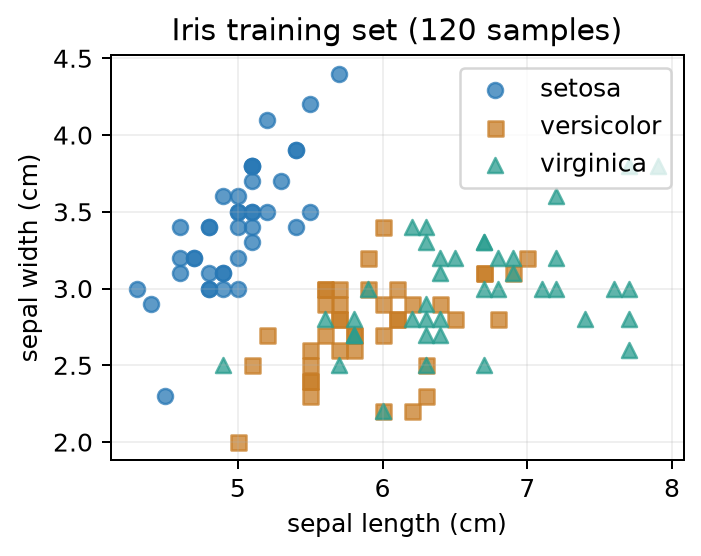
\includegraphics[width=0.48\linewidth]{assets/iris_sepal.png}\hfill
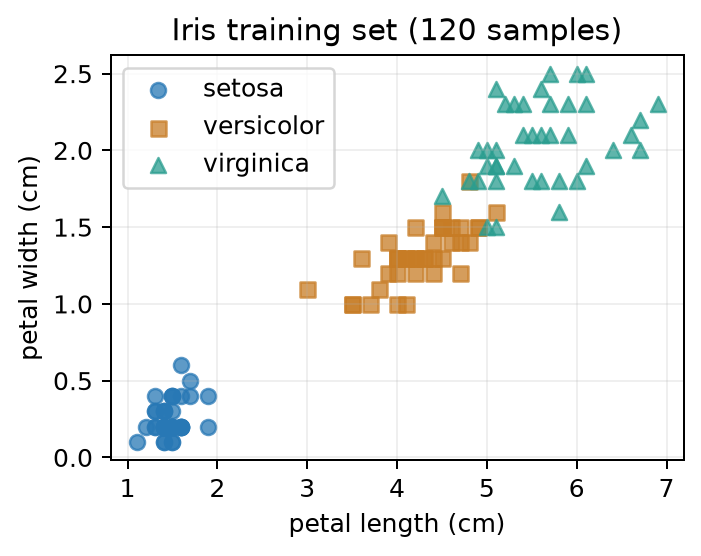
\includegraphics[width=0.48\linewidth]{assets/iris_petal.png}
\end{center}

左图使用花萼长、宽，右图使用花瓣长、宽；两图均为固定种子 42 的 120 个训练样本，每类 40 个。重合的点可能互相遮挡，因此图中肉眼数出的点数不一定是样本数。蓝色圆点为 setosa，橙色方点为 versicolor，绿色三角为 virginica。

右图中 setosa 更容易与另外两类分开；其余两类仍有重叠。这提示不同特征对当前分类问题提供的信息不同，但不是测试准确率，也不是因果结论。不能只凭图就宣称``花瓣特征一定是最佳特征''。

项目中的 \passthrough{\lstinline!draw\_scatter!} 已完整提供，用循环逐类筛选样本，再设置图例和坐标。若在 \passthrough{\lstinline!code!} 目录中新建 Notebook，可导入这个函数；接着前面的数据划分运行，修改列编号即可观察不同特征：

\begin{lstlisting}[language=Python]
import matplotlib.pyplot as plt
from iris.iris_classification import draw_scatter

draw_scatter(X_train, y_train, 0, 1,
             iris.feature_names, iris.target_names)
plt.show()
\end{lstlisting}

\textbf{动手 V1（约 5 分钟）：} 将图改为花萼长度与花瓣长度，说明哪一列作横轴、哪一列作纵轴，并写一句观察。Hint：修改调用中的列编号，不改数据划分，不把测试样本加到图里。

\clearpage

\subsection{直方图：范围、集中程度和区间数量 *}\label{ux76f4ux65b9ux56feux8303ux56f4ux96c6ux4e2dux7a0bux5ea6ux548cux533aux95f4ux6570ux91cf}

散点图看两个特征的关系，直方图看一个特征的分布。下面用训练集花瓣长度画图；\passthrough{\lstinline!X\_train[:, 2]!} 是所有训练行的第 3 列。

\begin{lstlisting}[language=Python]
plt.figure(figsize=(5.5, 3.5))
counts, edges, bars = plt.hist(
    X_train[:, 2], bins=10, color="#2878B5", edgecolor="white"
)
plt.xlabel("petal length (cm)")
plt.ylabel("Number of training samples")
plt.title("Petal length distribution")
plt.tight_layout()
plt.show()
\end{lstlisting}

\passthrough{\lstinline!figure!} 新建图，\passthrough{\lstinline!hist!} 把数值分到若干区间，\passthrough{\lstinline!bins=10!} 表示十个区间；\passthrough{\lstinline!counts!} 保存各区间样本数，\passthrough{\lstinline!edges!} 是区间边界，\passthrough{\lstinline!bars!} 是绘出的柱形对象，本课只检查 \passthrough{\lstinline!counts!}。横轴是长度，纵轴是频数，不是标签值，也不是分类概率。

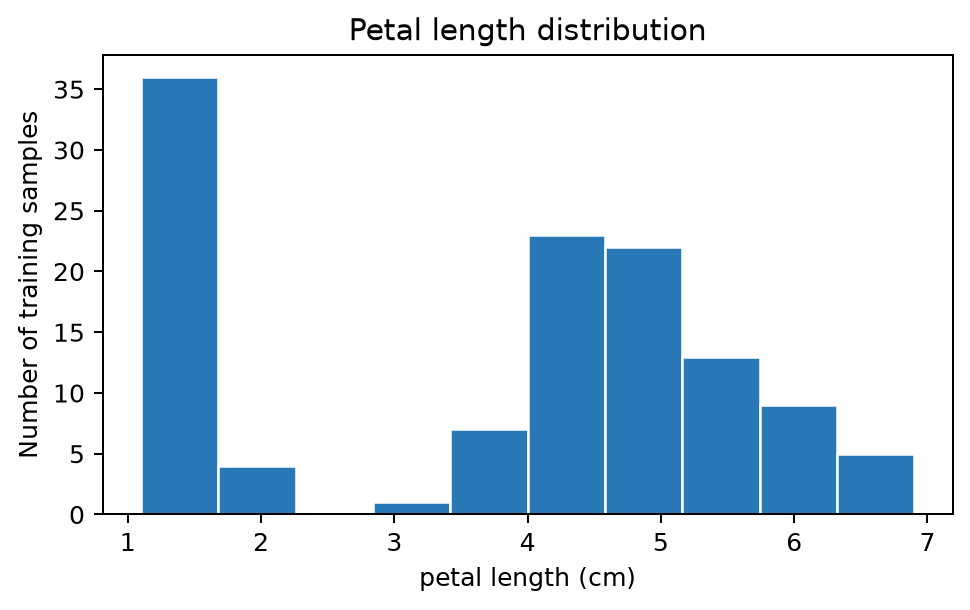
\includegraphics[width=0.68\linewidth,height=\textheight,keepaspectratio]{assets/iris_histogram.png}

图：训练集花瓣长度直方图，120 个样本、10 个区间。

图中的短花瓣与较长花瓣分布不均匀，但仅凭这张未按类别分组的图，不能给每根柱子直接指定品种。先描述``哪里多、哪里少、范围多大''，再回到散点图对照类别。

\textbf{动手 V2（约 4 分钟）：} 将 \passthrough{\lstinline!bins!} 改成 5、20，再比较图形。\passthrough{\lstinline!np.sum(counts)!} 应仍为 120。区间数量改变了呈现粒度，不会增加样本、改善模型或改变原始测量值。记录一张图与一句解释即可。

脚本的 \passthrough{\lstinline!plt.show()!} 可能等待图窗关闭才继续；Notebook 通常在单元下方显示。图使用英文标签以免不同电脑缺少中文字体。没有图窗的远程平台优先运行 Notebook；需要保存图片可用图窗保存按钮，注意不要覆盖已有文件。

\clearpage

\subsection{特征工程：选择、构造和缩放不是一回事 *}\label{ux7279ux5f81ux5de5ux7a0bux9009ux62e9ux6784ux9020ux548cux7f29ux653eux4e0dux662fux4e00ux56deux4e8b}

特征工程是把已有数据整理为模型可用的表示。先问``这个量对任务意味着什么''，再写变换。本次只做三步，不引入复杂自动搜索：

\begin{longtable}[]{@{}lll@{}}
\toprule\noalign{}
操作 & 具体做法 & 要回答的问题 \\
\midrule\noalign{}
\endhead
\bottomrule\noalign{}
\endlastfoot
选择 & 从原四列取花瓣长、宽两列 & 保留了什么，舍弃了什么？ \\
构造 & 追加花瓣长乘以宽 & 新量有何含义，单位是什么？ \\
缩放 & 使用训练均值、标准差标准化 & 规则从哪里估计，测试时怎样用？ \\
\end{longtable}

这里预先指定这两列用于教学，而不是根据测试准确率自动挑选。新特征``长×宽''只是花瓣大小的粗略代理，单位为平方厘米，不是真实花瓣面积；它是原数据的确定性组合，并没有采集新信息，也不保证提高准确率。

\begin{lstlisting}[language=Python]
train_petals = X_train[:, [2, 3]]
test_petals = X_test[:, [2, 3]]
train_area = train_petals[:, 0] * train_petals[:, 1]
test_area = test_petals[:, 0] * test_petals[:, 1]
X_train_features = np.column_stack((train_petals, train_area))
X_test_features = np.column_stack((test_petals, test_area))
\end{lstlisting}

\passthrough{\lstinline![:, [2, 3]]!} 按指定次序取两列；\passthrough{\lstinline!column\_stack!} 按列拼接，得到训练形状 \passthrough{\lstinline!(120, 3)!}、测试形状 \passthrough{\lstinline!(30, 3)!}，列顺序都是长度、宽度、长乘宽。训练与测试必须使用同一公式，不能只给训练集追加一列。

\textbf{手算例子：} 假设某朵花瓣长 4.0 cm、宽 1.5 cm，则新一行为 \passthrough{\lstinline![4.0, 1.5, 6.0]!}，第三项为 4.0×1.5。此为人工教学数值，不称作数据集某一行的测量结果。

\begin{lstlisting}[language=Python]
feature_scaler = StandardScaler()
train_scaled = feature_scaler.fit_transform(X_train_features)
test_scaled = feature_scaler.transform(X_test_features)
print(feature_scaler.mean_, feature_scaler.scale_)
print(np.mean(train_scaled, axis=0))
print(np.std(train_scaled, axis=0))
\end{lstlisting}

三个非恒定训练列变换后均值约为 0、标准差约为 1，测试集不必满足这一点。标准化不保证数值落在 0--1，也不使分布自动变成正态。当前决策树不要求缩放，本练习为后续距离模型与梯度优化准备。

\textbf{动手 F1/F2（约 7 分钟）：} 解释三个输出列及其单位；使用输出的训练均值和标准差，按``原值减均值，再除以标准差''复核首行首列。Hint：读取 \passthrough{\lstinline!X\_train\_features[0, 0]!}、\passthrough{\lstinline!feature\_scaler.mean\_[0]!} 和 \passthrough{\lstinline!feature\_scaler.scale\_[0]!}。

本文件只准备并检查新特征，不改变前面四特征决策树基线，也不承诺特征越多越好。若之后用新特征训练，训练与预测都要使用相同处理后的三列。要比较特征方案，须从训练部分留出验证集；测试集不参与选择。

\clearpage

\subsection{选读：清洗数据与避免泄漏 *}\label{ux9009ux8bfbux6e05ux6d17ux6570ux636eux4e0eux907fux514dux6cc4ux6f0f}

真实数据可能存在缺失、单位不一致或类别文本，需要按任务处理。本课已有数据完整，不强行制造``大型清洗流程''。下面专门用人工小表演示缺失值填补，与原鸢尾花数据区分：

\begin{lstlisting}[language=Python]
from sklearn.impute import SimpleImputer

toy_train = np.array([[1.0, 10.0], [2.0, np.nan], [3.0, 30.0]])
toy_test = np.array([[np.nan, 40.0]])
imputer = SimpleImputer(strategy="mean")
toy_train_filled = imputer.fit_transform(toy_train)
toy_test_filled = imputer.transform(toy_test)
print(imputer.statistics_)  # [2. 20.]
print(toy_test_filled)      # [[2. 40.]]
\end{lstlisting}

\passthrough{\lstinline!np.nan!} 表示缺失，不能直接当作 0。训练第一列均值为 2，第二列忽略缺失后的均值为 20；因此用 20 填补训练缺失值，用 2 填补测试缺失值。测试中的 40 不参与估计填补规则。均值填补只是一个简单策略，会改变数据分布，不适合不加判断地套用到所有任务。

\begin{longtable}[]{@{}ll@{}}
\toprule\noalign{}
情况 & 第一课应建立的判断 \\
\midrule\noalign{}
\endhead
\bottomrule\noalign{}
\endlastfoot
某列有缺失 & 先统计缺失数量，确认原因，再考虑填补或删除 \\
单位不一致 & 先统一含义与单位，不靠标准化掩盖录入问题 \\
类别为文字 & 模型常需编码；无序类别不能随意当成有大小的数值 \\
数值异常大 & 先核对记录和业务含义，不见到极端值就删除 \\
处理规则要从数据学习 & 只用训练部分估计，再应用到验证和测试部分 \\
\end{longtable}

数据泄漏不限于把 \passthrough{\lstinline!y\_test!} 传给模型。先用全部数据估计均值、根据测试集图形反复选特征、用答案衍生一列``特征''，都会让评价失去应有的独立性。看图并非无条件安全，因此本课探索图始终使用训练集。

\textbf{退出问题：} 现在得到三列标准化特征，能否直接拿它们交给此前用四列训练的模型预测？不能。列数、含义和处理规则都必须与模型训练时一致。要使用新表示，需在新表示上重新训练，并按验证与测试的职责评价。

缺失填补和类别编码本次不增加必交题。先能解释图、列、变换与训练边界，比调用更多库函数重要。

\clearpage

\section{复习、选读与查阅}\label{ux590dux4e60ux9009ux8bfbux4e0eux67e5ux9605}

\subsection{按需自查}\label{ux6309ux9700ux81eaux67e5}

\begin{enumerate}
\def\labelenumi{\arabic{enumi}.}
\tightlist
\item
  \passthrough{\lstinline!print!} 和 \passthrough{\lstinline!return!} 的区别是什么？给一个自己的例子。
\item
  价格是 \passthrough{\lstinline!"32.0"!} 时，为什么不能直接与数值相加？
\item
  三行三列的销量数组乘三元素价格数组，为什么只得到三个收入数值？
\item
  \passthrough{\lstinline!Book!} 与 \passthrough{\lstinline!first\_book!}、\passthrough{\lstinline!DecisionTreeClassifier!} 与 \passthrough{\lstinline!model!} 分别是什么关系？
\item
  \passthrough{\lstinline!fit!} 与 \passthrough{\lstinline!predict!} 做的事情有什么不同？测试标签能否用于训练？
\end{enumerate}

基础操作可在 \passthrough{\lstinline!practice.ipynb!} 中运行、修改和观察，不要求提交。正式成果来自两个微项目：书店代码通过分阶段验证，鸢尾花代码通过调用检查并产生实际结果。提交目录和 PDF 报告内容以实验手册为准。

\subsection{教学主题与材料入口}\label{ux6559ux5b66ux4e3bux9898ux4e0eux6750ux6599ux5165ux53e3}

\begin{longtable}[]{@{}
  >{\raggedright\arraybackslash}p{(\linewidth - 2\tabcolsep) * \real{0.5000}}
  >{\raggedright\arraybackslash}p{(\linewidth - 2\tabcolsep) * \real{0.5000}}@{}}
\toprule\noalign{}
\begin{minipage}[b]{\linewidth}\raggedright
主题
\end{minipage} & \begin{minipage}[b]{\linewidth}\raggedright
本次处理
\end{minipage} \\
\midrule\noalign{}
\endhead
\bottomrule\noalign{}
\endlastfoot
环境、数据类型、分支循环、函数 & 手册准备环境，practice.ipynb 运行基础例子 \\
文件、报错、NumPy & 讲义查阅，书店项目中组合应用 \\
元组、while、模块 & 选读小例子，遇到时再查 \\
类与继承 & Book 管理图书状态，CSVReader 的子类分别解析记录 \\
scikit-learn & 鸢尾花项目补全调用并验证，不要求手写算法 \\
异常捕获 & 选读一个 \passthrough{\lstinline!ValueError!} 例子，不要求给全部函数加检查 \\
时间测量 & 选读 \passthrough{\lstinline!perf\_counter!}，记录真实耗时，不背固定数字 \\
\end{longtable}

材料按概念、短练习和微项目相互连接，不要求逐项提交所有观察。先按手册完成依赖安装，再运行所需文件。

\clearpage

\subsection{记号与语法索引}\label{ux8bb0ux53f7ux4e0eux8bedux6cd5ux7d22ux5f15}

\begin{longtable}[]{@{}
  >{\raggedright\arraybackslash}p{(\linewidth - 4\tabcolsep) * \real{0.3333}}
  >{\raggedright\arraybackslash}p{(\linewidth - 4\tabcolsep) * \real{0.3333}}
  >{\raggedright\arraybackslash}p{(\linewidth - 4\tabcolsep) * \real{0.3333}}@{}}
\toprule\noalign{}
\begin{minipage}[b]{\linewidth}\raggedright
类别
\end{minipage} & \begin{minipage}[b]{\linewidth}\raggedright
记号
\end{minipage} & \begin{minipage}[b]{\linewidth}\raggedright
含义与首次说明位置
\end{minipage} \\
\midrule\noalign{}
\endhead
\bottomrule\noalign{}
\endlastfoot
数据与容器 & \passthrough{\lstinline!str!}、\passthrough{\lstinline!float!}、\passthrough{\lstinline!int!}、\passthrough{\lstinline!bool!} & 字符串、浮点数、整数、布尔值；第 2.1 节 \\
数据与容器 & \passthrough{\lstinline!list!}、\passthrough{\lstinline!dict!} & 列表、字典；第 2.2 节 \\
比较与赋值 & \passthrough{\lstinline!=!}、\passthrough{\lstinline!==!}、\passthrough{\lstinline!<=!} & 赋值、相等、不超过；第 2.1、3.1 节 \\
流程与函数 & \passthrough{\lstinline!for!}、\passthrough{\lstinline!if!}、\passthrough{\lstinline!return!} & 重复、判断、返回；第 3 节 \\
文件 & \passthrough{\lstinline!with open!} & 在代码块内使用并自动关闭文件；第 5.1 节 \\
数组计算 & \passthrough{\lstinline!np!}、\passthrough{\lstinline!shape!}、\passthrough{\lstinline!*!}、\passthrough{\lstinline!@!}、\passthrough{\lstinline!axis!} & 导入别名、形状、逐项乘法、矩阵乘法、计算轴；第 6.1--6.3 节 \\
对象 & \passthrough{\lstinline!class!}、\passthrough{\lstinline!self!}、\passthrough{\lstinline!\_\_init\_\_!} & 类、当前对象、初始化方法；第 7.1 节 \\
对象关系 & \passthrough{\lstinline!super()!}、\passthrough{\lstinline!isinstance!} & 调用父类实现、检查实例关系；第 7.3--7.4 节 \\
模型 & \passthrough{\lstinline!X!}、\passthrough{\lstinline!y!}、\passthrough{\lstinline!fit!}、\passthrough{\lstinline!predict!} & 特征、标签、训练、预测；第 8 节 \\
数据探索 & \passthrough{\lstinline!plt!}、\passthrough{\lstinline!bins!}、\passthrough{\lstinline!column\_stack!} & 绘图模块别名、区间数、按列拼接；第 8.7--8.9 节 \\
\end{longtable}

\subsection{实际使用的资料}\label{ux5b9eux9645ux4f7fux7528ux7684ux8d44ux6599}

\begin{itemize}
\tightlist
\item
  本课\href{code/bookstore/README.md}{书店项目}与\href{code/iris/README.md}{鸢尾花项目}的说明、学生代码、辅助模块与独立验证程序。
\item
  基础练习 \passthrough{\lstinline!code/practice.ipynb!}；文本读取示例数据 \passthrough{\lstinline!code/books.txt!}。
\item
  \href{https://docs.python.org/zh-cn/3.11/tutorial/introduction.html}{Python 官方教程：速览}与\href{https://docs.python.org/zh-cn/3.11/tutorial/controlflow.html}{控制流}，用于核对基础语法。
\item
  \href{https://docs.python.org/3.11/tutorial/classes.html}{Python 官方教程：类}，用于核对实例、类属性与继承语义。
\item
  \href{https://numpy.org/doc/stable/user/absolute_beginners.html}{NumPy 初学者指南}，用于核对数组、形状与轴的用法。
\item
  本课 \passthrough{\lstinline!code/iris/iris\_classification.py!}；\href{https://scikit-learn.org/stable/getting_started.html}{scikit-learn 入门}、\href{https://scikit-learn.org/stable/modules/generated/sklearn.datasets.load_iris.html}{鸢尾花数据接口}及\href{https://scikit-learn.org/stable/modules/generated/sklearn.model_selection.train_test_split.html}{数据划分接口}。
\item
  \href{https://scikit-learn.org/stable/modules/generated/sklearn.preprocessing.StandardScaler.html}{StandardScaler 官方接口}，用于核对训练统计量与变换的使用方式。
\item
  本章数据可视化示例；\href{https://matplotlib.org/stable/api/_as_gen/matplotlib.pyplot.scatter.html}{Matplotlib 散点图}与\href{https://matplotlib.org/stable/api/_as_gen/matplotlib.pyplot.hist.html}{直方图}，用于核对图形接口。
\item
  \href{https://scikit-learn.org/stable/common_pitfalls.html}{数据泄漏说明}与\href{https://scikit-learn.org/stable/modules/generated/sklearn.impute.SimpleImputer.html}{SimpleImputer 接口}，用于核对数据处理的训练边界。
\item
  \href{https://scikit-learn.org/stable/modules/generated/sklearn.tree.DecisionTreeClassifier.html}{决策树分类器接口}与\href{https://scikit-learn.org/stable/modules/generated/sklearn.metrics.confusion_matrix.html}{混淆矩阵接口}，用于核对概率列顺序、评价接口与矩阵方向。
\end{itemize}

案例与练习为课程自编，不将它们标为教材原题。

% 相关阅读位置：教材附录 A.1、A.2（书内第 276、279 页），第 3.1.5 节（第 76–78 页），第 5.2 节（第 159–160 页）；实验指导书第 1.5.2 节（第 9–10 页）、第 4.5.1 节（第 43–44 页）、第 7.5.2 节（第 103–104 页）及第 10 章第 147 页。上述页码均为书内印刷页码。

\end{document}
